\documentclass[a4paper,12pt,twoside]{memoir}

% Castellano
\usepackage[spanish,es-tabla]{babel}
\selectlanguage{spanish}
\usepackage[utf8]{inputenc}
\usepackage[T1]{fontenc}
\usepackage{lmodern} % Scalable font
\usepackage{microtype}
\usepackage{placeins}

\RequirePackage{booktabs}
\RequirePackage[table]{xcolor}
\RequirePackage{xtab}
\RequirePackage{multirow}

%Extras
\usepackage{graphicx}
\usepackage[bottom]{footmisc}

% Links
\PassOptionsToPackage{hyphens}{url}\usepackage[colorlinks]{hyperref}
\hypersetup{
	allcolors = {red}
}

% Ecuaciones
\usepackage{amsmath}

% Rutas de fichero / paquete
\newcommand{\ruta}[1]{{\sffamily #1}}

% Párrafos
\nonzeroparskip

% Huérfanas y viudas
\widowpenalty100000
\clubpenalty100000

% Imagenes
\usepackage{graphicx}
\newcommand{\imagen}[2]{
	\begin{figure}[!h]
		\centering
		\includegraphics[width=0.9\textwidth]{#1}
		\caption{#2}\label{fig:#1}
	\end{figure}
	\FloatBarrier
}

\newcommand{\imagenflotante}[2]{
	\begin{figure}%[!h]
		\centering
		\includegraphics[width=0.9\textwidth]{#1}
		\caption{#2}\label{fig:#1}
	\end{figure}
}



% El comando \figura nos permite insertar figuras comodamente, y utilizando
% siempre el mismo formato. Los parametros son:
% 1 -> Porcentaje del ancho de página que ocupará la figura (de 0 a 1)
% 2 --> Fichero de la imagen
% 3 --> Texto a pie de imagen
% 4 --> Etiqueta (label) para referencias
% 5 --> Opciones que queramos pasarle al \includegraphics
% 6 --> Opciones de posicionamiento a pasarle a \begin{figure}
\newcommand{\figuraConPosicion}[6]{%
  \setlength{\anchoFloat}{#1\textwidth}%
  \addtolength{\anchoFloat}{-4\fboxsep}%
  \setlength{\anchoFigura}{\anchoFloat}%
  \begin{figure}[#6]
    \begin{center}%
      \Ovalbox{%
        \begin{minipage}{\anchoFloat}%
          \begin{center}%
            \includegraphics[width=\anchoFigura,#5]{#2}%
            \caption{#3}%
            \label{#4}%
          \end{center}%
        \end{minipage}
      }%
    \end{center}%
  \end{figure}%
}

%
% Comando para incluir imágenes en formato apaisado (sin marco).
\newcommand{\figuraApaisadaSinMarco}[5]{%
  \begin{figure}%
    \begin{center}%
    \includegraphics[angle=90,height=#1\textheight,#5]{#2}%
    \caption{#3}%
    \label{#4}%
    \end{center}%
  \end{figure}%
}
% Para las tablas
\newcommand{\otoprule}{\midrule [\heavyrulewidth]}
%
% Nuevo comando para tablas pequeñas (menos de una página).
\newcommand{\tablaSmall}[5]{%
 \begin{table}
  \begin{center}
   \rowcolors {2}{gray!35}{}
   \begin{tabular}{#2}
    \toprule
    #4
    \otoprule
    #5
    \bottomrule
   \end{tabular}
   \caption{#1}
   \label{tabla:#3}
  \end{center}
 \end{table}
}

%
% Nuevo comando para tablas pequeñas (menos de una página).
\newcommand{\tablaSmallSinColores}[5]{%
 \begin{table}[H]
  \begin{center}
   \begin{tabular}{#2}
    \toprule
    #4
    \otoprule
    #5
    \bottomrule
   \end{tabular}
   \caption{#1}
   \label{tabla:#3}
  \end{center}
 \end{table}
}

\newcommand{\tablaApaisadaSmall}[5]{%
\begin{landscape}
  \begin{table}
   \begin{center}
    \rowcolors {2}{gray!35}{}
    \begin{tabular}{#2}
     \toprule
     #4
     \otoprule
     #5
     \bottomrule
    \end{tabular}
    \caption{#1}
    \label{tabla:#3}
   \end{center}
  \end{table}
\end{landscape}
}

%
% Nuevo comando para tablas grandes con cabecera y filas alternas coloreadas en gris.
\newcommand{\tabla}[6]{%
  \begin{center}
    \tablefirsthead{
      \toprule
      #5
      \otoprule
    }
    \tablehead{
      \multicolumn{#3}{l}{\small\sl continúa desde la página anterior}\\
      \toprule
      #5
      \otoprule
    }
    \tabletail{
      \hline
      \multicolumn{#3}{r}{\small\sl continúa en la página siguiente}\\
    }
    \tablelasttail{
      \hline
    }
    \bottomcaption{#1}
    \rowcolors {2}{gray!35}{}
    \begin{xtabular}{#2}
      #6
      \bottomrule
    \end{xtabular}
    \label{tabla:#4}
  \end{center}
}

%
% Nuevo comando para tablas grandes con cabecera.
\newcommand{\tablaSinColores}[6]{%
  \begin{center}
    \tablefirsthead{
      \toprule
      #5
      \otoprule
    }
    \tablehead{
      \multicolumn{#3}{l}{\small\sl continúa desde la página anterior}\\
      \toprule
      #5
      \otoprule
    }
    \tabletail{
      \hline
      \multicolumn{#3}{r}{\small\sl continúa en la página siguiente}\\
    }
    \tablelasttail{
      \hline
    }
    \bottomcaption{#1}
    \begin{xtabular}{#2}
      #6
      \bottomrule
    \end{xtabular}
    \label{tabla:#4}
  \end{center}
}

%
% Nuevo comando para tablas grandes sin cabecera.
\newcommand{\tablaSinCabecera}[5]{%
  \begin{center}
    \tablefirsthead{
      \toprule
    }
    \tablehead{
      \multicolumn{#3}{l}{\small\sl continúa desde la página anterior}\\
      \hline
    }
    \tabletail{
      \hline
      \multicolumn{#3}{r}{\small\sl continúa en la página siguiente}\\
    }
    \tablelasttail{
      \hline
    }
    \bottomcaption{#1}
  \begin{xtabular}{#2}
    #5
   \bottomrule
  \end{xtabular}
  \label{tabla:#4}
  \end{center}
}



\definecolor{cgoLight}{HTML}{EEEEEE}
\definecolor{cgoExtralight}{HTML}{FFFFFF}

%
% Nuevo comando para tablas grandes sin cabecera.
\newcommand{\tablaSinCabeceraConBandas}[5]{%
  \begin{center}
    \tablefirsthead{
      \toprule
    }
    \tablehead{
      \multicolumn{#3}{l}{\small\sl continúa desde la página anterior}\\
      \hline
    }
    \tabletail{
      \hline
      \multicolumn{#3}{r}{\small\sl continúa en la página siguiente}\\
    }
    \tablelasttail{
      \hline
    }
    \bottomcaption{#1}
    \rowcolors[]{1}{cgoExtralight}{cgoLight}

  \begin{xtabular}{#2}
    #5
   \bottomrule
  \end{xtabular}
  \label{tabla:#4}
  \end{center}
}



\graphicspath{ {./img/} }

% Capítulos
\chapterstyle{bianchi}
\newcommand{\capitulo}[2]{
	\setcounter{chapter}{#1}
	\setcounter{section}{0}
	\setcounter{figure}{0}
	\setcounter{table}{0}
	\chapter*{#2}
	\addcontentsline{toc}{chapter}{#2}
	\markboth{#2}{#2}
}

% Apéndices
\renewcommand{\appendixname}{Apéndice}
\renewcommand*\cftappendixname{\appendixname}

\newcommand{\apendice}[1]{
	%\renewcommand{\thechapter}{A}
	\chapter{#1}
}

\renewcommand*\cftappendixname{\appendixname\ }

% Formato de portada
\makeatletter
\usepackage{xcolor}
\newcommand{\tutor}[1]{\def\@tutor{#1}}
\newcommand{\course}[1]{\def\@course{#1}}
\definecolor{cpardoBox}{HTML}{E6E6FF}
\def\maketitle{
  \null
  \thispagestyle{empty}
  % Cabecera ----------------
\noindent
\includegraphics[width=\textwidth]{cabecera}\vspace{1cm}%
  \vfill
  % Título proyecto y escudo informática ----------------
  \colorbox{cpardoBox}{%
    \begin{minipage}{.8\textwidth}
      \vspace{.5cm}\Large
      \begin{center}
      \textbf{TFG del Grado en Ingeniería Informática}\vspace{.6cm}\\
      \textbf{\LARGE\@title{}}
      \end{center}
      \vspace{.2cm}
    \end{minipage}

  }%
  \hfill\begin{minipage}{.20\textwidth}
    
\includegraphics[width=\textwidth]{escudoInfor}
  \end{minipage}
  \vfill
  % Datos de alumno, curso y tutores ------------------
  \begin{center}%
  {%
    \noindent\LARGE
    Presentado por \@author{}\\ 
    en Universidad de Burgos --- \@date{}\\
    Tutor: \@tutor{}\\
  }%
  \end{center}%
  \null
  \cleardoublepage
  }
\makeatother

\newcommand{\nombre}{Marcos Romano Ibáñez} %%% cambio de comando

% Datos de portada
\title{Desarrollo de un videojuego del género Plataformas 2D en Unity}
\author{\nombre}
\tutor{Jesús María Alonso Abad}
\date{\today}

\begin{document}

\maketitle


\newpage\null\thispagestyle{empty}\newpage


%%%%%%%%%%%%%%%%%%%%%%%%%%%%%%%%%%%%%%%%%%%%%%%%%%%%%%%%%%%%%%%%%%%%%%%%%%%%%%%%%%%%%%%%
\thispagestyle{empty}


\noindent
\includegraphics[width=\textwidth]{cabecera}\vspace{1cm}

\noindent D. nombre tutor, profesor del departamento de nombre departamento, área de nombre área.

\noindent Expone:

\noindent Que el alumno D. \nombre, con DNI 71310718T, ha realizado el Trabajo final de Grado en Ingeniería Informática titulado ''Desarrollo de un videojuego del género Plataformas 2D en Unity''. 

\noindent Y que dicho trabajo ha sido realizado por el alumno bajo la dirección del que suscribe, en virtud de lo cual se autoriza su presentación y defensa.

\begin{center} %\large
En Burgos, {\large \today}
\end{center}

\vfill\vfill\vfill

% Author and supervisor
%\begin{minipage}{0.45\textwidth}
%\begin{flushleft} %\large
%Vº. Bº. del Tutor:\\[2cm]
%D. nombre tutor
%\end{flushleft}
%\end{minipage}
%\hfill
%\begin{minipage}{0.45\textwidth}
%\begin{flushleft} %\large
%Vº. Bº. del co-tutor:\\[2cm]
%D. nombre co-tutor
%\end{flushleft}
%\end{minipage}
%\hfill

%\vfill

%para casos con solo un tutor comentar lo anterior
%y descomentar lo siguiente
Vº. Bº. del Tutor:\\[2cm]
Jesús María Alonso Abad


\newpage\null\thispagestyle{empty}\newpage




\frontmatter

% Abstract en castellano
\renewcommand*\abstractname{Resumen}
\begin{abstract}
La intención de este trabajo va a ser el desarrollo de un videojuego de plataformas 2D con el motor de videojuegos Unity y el lenguaje de programación C\#.

Las principales mecánicas del juego consistirán en influir sobre la física y el tiempo para ayudar o dificultar que el jugador supere los niveles del juego.

\end{abstract}

\renewcommand*\abstractname{Descriptores}
\begin{abstract}
Videojuegos, plataformas 2D, Unity, C\#
\end{abstract}

\clearpage

% Abstract en inglés
\renewcommand*\abstractname{Abstract}
\begin{abstract}
The intention of this work will be to develop a 2D platformer video game with the Unity game engine and the C\# programming languaje.

The main mechanics of the game will consist of manipulating physics and time to help or obstruct the player to pass the levels of the game.

\end{abstract}

\renewcommand*\abstractname{Keywords}
\begin{abstract}
Video game, Platformer 2D, Unity, C\#
\end{abstract}

\clearpage

% Indices
\tableofcontents

\clearpage

\listoffigures

\clearpage

%\listoftables
%\clearpage

\mainmatter
\capitulo{1}{Introducción}

Los videojuegos son productos software enfocados al ocio. Desde el primer videojuego, el \textit{Tennis for Two \cite{Tennis4two}} creado en 1958 por el físico William Higginbotham hasta los juego actuales, estos han ido creciendo en calidad y envergadura hasta convertirse la industria de los videojuegos en una de las que más dinero mueve habiendo recaudado en 2020 entorno a 140.000 millones de dólares \cite{2020GamesMoney}.

Sin embargo, los videojuegos son productos software muy particulares intrínsecamente relacionados con otros ámbitos del ocio como la música o el arte visual. Debido a la curiosidad que genera este producto tan complejo y el amor que se profesa por los videojuegos se ha decidido desarrollar un videojuego con el objetivo de entender cual es el funcionamiento interno de un videojuego y como es su desarrollo como producto software.

Se plantearán las mecánicas y elementos que tendrá el videojuego. Una vez decidido esto, se generará un documento de diseño de juego con toda la información relativa al producto que se desea lograr y de lo que estará compuesto. El documento de diseño de juego tendrá un lenguaje coloquial pero su importancia radica en lo útil que resulta para marcar el rumbo del proceso de creación del juego y ofrecer una visión de lo que acabará siendo el videojuego.

Con el documento de diseño de juego creado se procederá a desarrollar el videojuego con el objetivo de alcanzar las metas establecidas en este.

\section{Materiales Adjuntos}
Este TFG consta de los siguientes materiales:
\begin{itemize}
\item
La memoria del TFG.
\item
Los anexos (el documento de diseño de juego estará redactado en los anexos).
\item
La solución de Visual Studio que contiene el código en C\# correspondiente al videojuego.
\item
El fichero comprimido con el sistema de ficheros y el ejecutable que hará funcionar el juego en ordenador.
\item
El fichero comprimido con el sistema de ficheros y el ejecutable que permita ejecutar el juego en WebGL.
\end{itemize}

Todos estos elementos serán accesibles a través del repositorio de GitHub: \url{https://github.com/Kencho/mri1001-tfg}

\section{Estructura de la memoria}
La memoria consta de los siguientes apartados:
\begin{itemize}
\item
\textbf{Introducción:} Resumen del motivo de este proyecto, materiales que conformará el producto y documentos relativos a este.
\item
\textbf{Objetivos del proyecto:} Explicación de los objetivos propuestos para el proyecto.
\item
\textbf{Conceptos teóricos:} Conocimiento teórico relativo al proyecto que introduce conceptos mencionados en los demás apartados que se darán por aprehendidos.
\item
\textbf{Técnicas y herramientas:} Técnicas y herramientas relativas al desarrollo del proyecto, en qué consisten y qué uso se les va a dar.
\item
\textbf{Aspectos relevantes del desarrollo:} Explicación de la implementación que se ha realizado sobre los elementos del videojuego.
\item
\textbf{Trabajos relacionados:} Proyectos relativos al videojuego que se está desarrollando, tanto como referencias como proyectos en los que inspirarse.
\item
\textbf{Conclusiones y líneas de trabajo futuras:} Conocimientos adquiridos, críticas a las herramientas utilizadas y próximas tareas relativas al proyecto.
\end{itemize}

\section{Anexos}
La memoria contará adicionalmente con los siguientes anexos:
\begin{itemize}
\item
\textbf{Plan de proyecto software:} Planificación temporal del desarrollo del proyecto y estudio de viabilidad de este.
\item
\textbf{Especificación de requisitos:} Especificación de requisitos y casos de uso.
\item
\textbf{Especificación de diseño:} Elementos relativos al diseño.
\item
\textbf{Documentación técnica de programación:} Estructura de ficheros y elementos de interés relativo al programador.
\item
\textbf{Documentación de usuario:} Información relativa a los usuarios de la aplicación y manual del usuario.
\item
\textbf{Documento de diseño del juego:} Documento de diseño del juego con la información relativa al videojuego que se desea desarrollar.
\end{itemize}
\capitulo{2}{Objetivos del proyecto}

El objetivo principal del proyecto será el desarrollo de un videojuego del género Plataformas 2D. De este objetivo principal derivan otros varios, tales como aprender el funcionamiento y estructura del motor de videojuegos Unity, que será el utilizado durante el desarrollo del videojuego. También se busca analizar, comprender e implementar los elementos que componen un videojuego de plataformas 2D y la arquitectura lógica que permite que funcione.

\capitulo{3}{Conceptos teóricos}

\section{Unity \cite{Unity}}
En este apartado se va a explicar que es Unity y algunos de los elementos que lo componen y de los que hace uso. Este apartado es importante porque durante toda la memoria se va a hacer referencia a estos elementos asumiendo que se ha leído este apartado.

Unity(1) es un motor gráfico orientado al desarrollo de videojuegos que permite desarrollar para ordenador (Microsoft Windows, Mac OS y Linux), consolas, móvil y dispositivos de realidad aumentada.

Unity tiene una serie de elementos, pero los más destacables son:

\subsection{MonoBehaviour}
MonoBehaviour es la clase de la que (en principio) parten todas las clases que utiliza Unity. Esta clase y sus hijas son las que inicializa Unity al crear una escena. La razón por la que esta clase es tan importante y requiere de explicación son los siguientes métodos:

\textbf{Awake() y Start():} Tanto Awake como Start son métodos que se ejecutan al crear un objeto que herede de MonoBehaviour, sin embargo funcionan de manera ligeramente distinta. 

El método Awake se llama en el instante exacto en el que se carga el script al que está asociado o en el que se crea la instancia del nuevo objeto de esta clase. Funciona prácticamente como el constructor de una clase. Es un método muy adecuado para inicializar variables ya que se ejecutará justo al crearse la instancia del objeto o cargarse el script. 

El método Awake se ejecutará siempre independientemente de que el objeto este activado o no. Con activado se hace referencia al atributo booleano enabled de la clase MonoBehaviour. Cuando este atributo este a false el objeto no realizará ninguna operación (actuará como si estuviese desactivado) y cuando este a true funcionará con normalidad.

Como se ha mencionado el método Start funciona de manera muy similar a Awake pero con dos diferencias clave. El método Start se activa antes de que se llame a cualquier método Update (explicados a continuación), pero no garantiza que se valla a llamar en el mismo momento en el que se crea el objeto o se carga el script (a diferencia del método Awake). La otra diferencia con Awake es que el método Start se llamará solo si el objeto esta activado (enabled a true) mientras que Awake se llamará siempre.\\


\textbf{Update(), FixedUpdate() y LateUpdate():} Estos tres son métodos que se llaman repetitivamente hasta la desaparición del objeto. Estos métodos son los que utilizará Unity para saber en todo momento que es lo que tiene que hacer y en qué momento ha de hacerlo. Pero ¿Por qué hacer tres métodos distintos para albergar instrucciones que se repetirán continuamente? La razón de esto reside en cuándo se ejecutan estos tres métodos.

El método Update se llama cada frame. Explicado a grandes rasgos un frame representa el momento en el que cambia lo que sale por pantalla. Así que cada vez que cambia lo que se ve en pantalla se llama al método Update. El tiempo que puede pasar entre frames no tiene por qué ser siempre el mismo. Es por ello que el periodo entre llamadas al método Update no siempre será el mismo.

El método FixedUpdate se llama repetitivamente, con la excepción de que no lo hace cada frame, sino que se repite en el tiempo de manera regular. El periodo entre llamadas al método FixedUpdate será siempre de 0.02 segundos. Este periodo se puede modificar pero la llamada al método Fixed Update siempre será regular. Esto hace al método FixedUpdate un método ideal para realizar cálculos dependientes del momento del tiempo en el que te halles (calcular trayectorias de objetos por ejemplo).

El método LateUpdate es muy similar al método Update. También se ejecuta en cada frame pero difiere del método Update en que se ejecutará siempre después de los demás métodos “update”. Esto puede ser útil para la actualización de elementos que requieren que se hayan hecho una serie de cambios antes. Un ejemplo podría ser el seguimiento de una cámara a un objeto. Si se establece el seguimiento de la cámara y luego se actualiza la posición del objeto la cámara va a estar persiguiendo al objeto en una posición en la que no está.\\


\textbf{Mensajes:} Además de estos métodos hay otros métodos que se identifican por el nombre de “mensajes”. Los “mensajes” funcionan de forma un poco diferente a los métodos normales y corrientes. Son métodos que se pueden activar con normalidad al llamarlos, pero también son métodos que se pueden activar al “recibir un mensaje” utilizando el método SendMessage() de la clase GameObject (esta clase se explicará a continuación). La gracia de estos métodos “mensaje” no está en que se encuentren en la clase MonoBehaviour, sino como interactúan con otras clases y objetos. Es por eso que a continuación se mencionarán los más interesantes, pero la explicación de los métodos se realizará en otro apartado en el que se haga referencia a estos métodos y se comprenda mejor el uso de estos.

Métodos “mensaje”:
\begin{itemize}
\item
OnCollisionEnter.
\item
OnCollisionEnter2D.
\item
OnCollisionExit.
\item
OnCollisionExit2D.
\item
OnCollisionStay.
\item
OnCollisionStay2D.
\item
OnTriggerEnter.
\item
OnTriggerEnter2D.
\item
OnTriggerExit.
\item
OnTriggerExit2D.
\item
OnTriggerStay.
\item
OnTriggerStay2D.
\item
Start (también es un método “mensaje”).
\item
Update (también es un método “mensaje”).
\end{itemize}

\subsection{GameObject}
La clase GameObject es la clase de la que parten todos los objetos que va a utilizar Unity. Todos los elementos que creas en Unity son GameObject. La clase GameObject por defecto añade atributos que ofrecen información básica sobre ese GameObject. Algunos de los más importantes serían: transform para saber qué región del espacio ocupa el GameObject, tag para identificar al GameObject y name para identificar tanto al GameObject como a los componentes de este (todos comparten el mismo nombre).
GameObject por si sola es una clase inútil. Pero lo importante de GameObject es la capacidad que posee para añadirse componentes a si mimo (con el método GetComponent entre otros). Los componentes, al ser añadidos a la instancia de GameObject que le corresponda ya pueden ser usados por Unity. Los componentes de GameObject pueden ser objetos de cualquier tipo, sin necesidad de heredar de MonoBehaviour.

GameObject posee varios métodos estáticos, pero se van a explicar dos que se creen dignos de mención. Estos métodos son Destroy e Instantiate. Lo que hacen estos métodos se puede deducir por el nombre de estos. Destroy destruye instancias de GameObject y/o componentes de estos y el método Instantiate las crea. Sn embargo, cabe mencionar que el método Instantiate no crea de verdad los objetos, sino que clona uno existente y devuelve el objeto clonado. Esto es importante porque Unity provee unos objetos especiales que son los Prefabs. Estos Prefabs son un GameObject persistente que guarda la configuración con la que ha sido construido ese GameObject. De esta manera si tienes un Prefab de, por ejemplo, un enemigo del juego puedes crear todas las copias de ese enemigo que quieras llamando al método Instantiate y pasando como argumento ese Prefab. Con los Prefabs se logra tener copias idénticas de objetos sin tener que crearlas manualmente cada vez.

La última característica importante de GameObject es el método SendMessage. Este método permite al GameObject o un componente suyo mandar un mensaje a los demás componentes del GameObject, haciendo que todos los componentes (en realidad solo los que hereden de MonoBehaviour) que tengan un método con nombre igual al pasado como argumento en el método SendMessage ejecutarán ese método. Un ejemplo sería gameobject.SendMessage(“Metodo1”). Al ejecutar ese método se hará que todos los componentes que hereden de MonoBehaviour y tengan un método llamado Metodo1 invoquen ese método.

\subsection{Escenas}
Las escenas son elementos de Unity que contienen otros objetos. Una escena puede ser un nivel o un menú del juego.

\subsection{Físicas en Unity}
Un objeto por defecto no se ve afectado por las físicas. Sin embargo añadiendo el componente Rigidbody (Rigidbody2D para los juegos en dos dimensiones) el GameObject al que este asociado variará su posición como si estuviese afectado por las físicas.

Rigidbody tiene un atributo llamado velocity. Este atributo un vector de 3 dimensiones que representa en qué dirección se moverá el GameObject afectado por las físicas. Un componente Rigidbody hace que su GameObject se vea afectado por la gravedad o no con el atributo booleano useGravity.

Rigidbody tiene un atributo booleano llamado isKinematic. Este atributo hace que un objeto no se vea afectado por las colisiones. Un objeto con un Rigidbody con el atributo isKinematic igual a true (objeto 1) que colisiona con otro con un Rigidbody con el atributo iskinematic igual a false (objeto 2) provoca que el objeto 1 modifique su movimiento teniendo en cuenta las reacciones físicas generadas por la colisión con el objeto 2. El objeto 2, sin embargo no verá su movimiento afectado por la colisión.

\subsection{Colisión entre objetos}
Unity ofrece por defecto una manera de manejar las colisiones entre objetos. Para que un GameObject ofrezca la posibilidad de colisionar con otro objeto, este debe de tener un componente llamado Collider (para los juegos en dos dimensiones Collider2D). Este componente te permite determinar una región del espacio en la que otro GameObject con un componente Collider se considerará colisionando con el primer objeto. Si dos Colliders comparten algún punto de los espacios que delimitan, se considerará que se ha producido una colisión entre los GameObject a los que pertenecen. 

La región del espacio que ocupa un Collider por defecto es estática y no se puede mover, sin embargo moviendo la posición del GameObject moverá la posición del Collider, pues su posición es relativa al GameObject.

La colisión entre objetos se desarrolla mediante la ejecución de los métodos OnCollisionEnter/Stay/Exit de los componentes que heredan de la clase MonoBehaviour que tengan implementados esos métodos. 
Si dos objetos tienen un Rigidbody y un Collider, al colisionar ambos objetos variaran su movimiento en consecuencia. Sin embargo, si se desea evitar esto, el componente Collider tiene un atributo booleano llamado isTrigger. Si está a false el funcionamiento será el explicado anteriormente. Sin embargo, si está a true el atributo isTrigger, su movimiento no se verá afectado al colisionar pero sí que se detectará la colisión. En caso de que el atributo isTrigger sea true, la colisión no se resolverá ejecutando los métodos anteriormente explicados, sino que se resolverá mediante los métodos OnTriggerEnter/Stay/Exit de los componentes que heredan de la clase MonoBehaviour que tengan implementados esos métodos.

\capitulo{4}{Técnicas y herramientas}

\section{Motor de videojuegos}
Para la creación del videojuego se planteó apoyarse en un motor de videojuegos ya creado frente a implementar todo el proyecto desde cero. Se planteó utilizar Unity (hacer uso de un motor de videojuegos) frente a la biblioteca de Python pygames (no hacer uso de un motor de videojuegos).

\subsection{Unity}
Para el desarrollo del videojuego se ha considerado utilizar Unity como motor de videojuegos, ya que es un motor de videojuegos gratuito de fácil uso (aunque limitado en algunos aspectos), pero que ofrece los recursos necesarios para el desarrollo. Esta herramienta trae elementos ya implementados que ahorran mucho tiempo de trabajo tales como los Colliders (clases encargadas del manejo de las colisiones entre objetos) y clases encargadas de simular las físicas e interactuar entre estas y los objetos en la escena. Además, Unity ofrece una interfaz que facilite la visualización de los niveles del videojuego.

El argumento final para elegir este motor de videojuegos y no otros como, por ejemplo, Unreal Engine 4 ha sido completamente subjetivo. Ya se tiene experiencia previa y se ahorrará mucho tiempo del que se invertiría en el proceso de aprendizaje de otro motor de videojuegos.

\subsection{Pygames (biblioteca de Python)}
Pygames es una herramienta que ofrece una serie de clases que ofrecen una solución intermedia entre construir desde cero todo el código relativo al desarrollo de un videojuego y un motor de videojuegos que ofrece bastantes elementos de un videojuego ya implementados. 

Construir desde cero el videojuego podría llevar demasiado tiempo y probablemente no diese tiempo a desarrollar el videojuego entero como un elemento funcional. Sin embargo, hacerlo desde cero ofrece una libertad absoluta en el desarrollo y la funcionalidad.
Utilizar un motor de videojuegos para el desarrollo del videojuego facilita mucho el desarrollo, sin embargo obliga a ceñirse al modelo que sigue el motor de videojuegos.

La biblioteca pygames ofrece una solución intermedia, ofreciendo bastante libertad y una estructura de clases que limita muy poco ofreciendo las funcionalidades justas y necesarias (creación de la ventana donde se mostrará el juego, visualización de sprites y elementos visuales y poco más).

\subsection{Decisión final}
Finalmente se ha optado por el uso del motor de videojuegos Unity en lugar de la biblioteca pygames porque es un entorno con el que se está más familiarizado (teniéndose un conocimiento mucho más profundo de Unity que de pygames). Como ya se ha mencionado anteriormente el proceso de aprendizaje puede llevar demasiado tiempo (puesto que para pygames se posee un conocimiento muy básico). Adicionalmente se teme que, al ser pygames demasiado abierto (una de sus ventajas), no se tenga tiempo suficiente para desarrollar un videojuego con el nivel de acabado que se ha propuesto para este proyecto en el tiempo del que se dispone.

Debido a su facilidad de uso y los elementos que ya trae por defecto se ha elegido Unity para el desarrollo del videojuego.


\capitulo{5}{Aspectos relevantes del desarrollo del proyecto}

\section{Arquitectura del Player}
Player es el GameObject asociado al avatar que controlará el jugador y posee un componente PlayerController. La clase PlayerController, se encarga del funcionamiento del objeto como avatar controlable por el jugador.

La clase PlayerController hereda de la clase KinematicObject. KinematicObject es una clase que hereda de MonoBehaviour y se encarga de simular la gravedad sobre el objecto y gestionar las colisiones contra obstáculos que puedan afectar al movimiento (se profundizará en este aspecto en el apartado de gestión de las colisiones).

\clearpage
\begin{figure}[h]
\centering
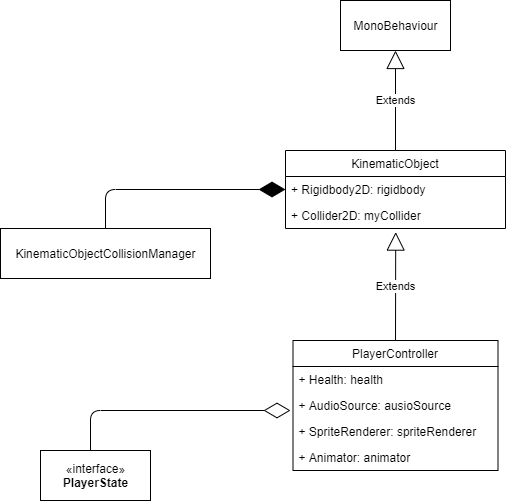
\includegraphics[scale=0.7]{Memoria/Aspectos_relevantes/Arquitectura_Player/Jerarqui_herencia_PlayerController}
\caption{Jerarquía de herencia de PlayerController}
\end{figure}

El PlayerController utiliza el patrón de diseño Estado, de manera que hay acciones generales que realiza la propia clase PlayerControler y otras que delega en las clases que heredan de la interfaz PlayerState
Las operaciones generales que realiza PlayerController son:
\begin{itemize}
\item
Para el método Update se encarga de la animación del personaje (de la parte más genérica) y de comprobar si algún botón o tecla asociado a una acción ha sido pulsado y se requiere alguna acción como respuesta (esa acción se ejecutará en el FixedUpdate).
\item
Para el método FixedUpdate se actualizan las banderas y en caso de haber pulsado el botón de salto o del acelerón se realiza la acción (si se puede realizar). Las banderas son una serie de variables booleanas que marcan si se pueden o no realizar acciones concretas. Las banderas son los booleanos que dictaminan si se puede o no ejecutar las mecánicas del Player.
\end{itemize}

\subsection{Estados del Player}
El Player se comportará de distinta forma en función de en que situación se encuentre. Para facilitar la lógica del Player y el cambio en tiempo de ejecución del comportamiento de este, se ha aplicado el patrón de diseño Estado.

\begin{figure}[h]
\centering
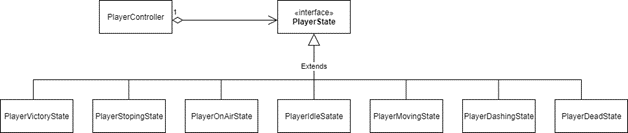
\includegraphics[scale=0.85]{Memoria/Aspectos_relevantes/Arquitectura_Player/Estados_Player}
\caption{Diagrama UML de la aplicación del patrón de diseño Estado en el Player}
\end{figure}

El Player puede estar en los siguientes estados:
\begin{itemize}
\item
PlayerIdleState: El Player está detenido sobre una superficie.
\item
PlayerOnAirState: El Player está en el aire.
\item
PlayerMovingState: El Player se está moviendo sobre una superficie.
\item
PlayerStopingState: El Player ha cesado el movimiento y se está deteniendo.
\item
PlayerDashingState: El Player está realizando el acelerón.
\item
PlayerVictoryState: El Player ha llegado a la meta.
\item
PlayerDeadState: El Player está muerto.
\end{itemize}

En el anexo C se da una explicación detallada de la implementación hecha del patrón de diseño estado.

\subsection{Interfaz PlayerMechanic}
Las mecánicas de salto, el acelerón y la mecánica de tiempo bala que puede realizar el Player han sido implementadas en tres clases que heredan de la interfaz PlayerMechanic. Esta interfaz incluye tres métodos: ManageInput para encargarse de comprobar si están pulsando los botones necesarios para llevar a cabo la mecánica, ManageFlags para gestionar los booleanos utilizados para saber si se va a llevar a cabo la mecánica o no, y ExecuteMechanic para ejecutar la mecánica (si se cumplen las condiciones necesarias para llevarla a cabo).

\begin{figure}[h]
\centering
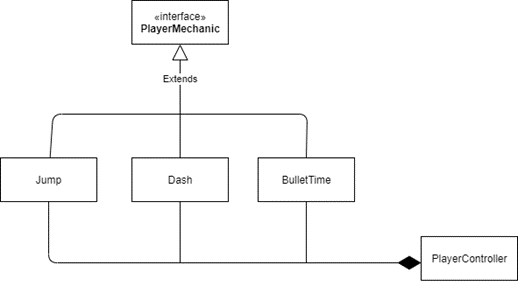
\includegraphics[scale=1]{Memoria/Aspectos_relevantes/Arquitectura_Player/PlayerMechanics}
\caption{Diagrama UML de la implementación de las mecánicas en PlayerController mediante composición}
\end{figure}

\section{Sistema de colisiones \cite{ContinuousCollision}\cite{UnderstandingConstraints}}
El objeto Player es un objeto con un Rigidbody2D kinemático. Para que dos objetos choquen al colisionar de manera ideal en el entorno de Unity es necesario que los objetos que colisionan tengan los componentes Collider y Rigidbody. Es necesario que el atributo BodyType del Rigidbody sea de tipo Dinamic. Cuando el Rigidbody es dinámico, Unity simula físicas sobre ese objeto. Como en el juego se va a trabajar con un sistema de físicas propio, el Rigidbody de los objetos con el componente KinematicObject no puede ser dinámico sino kinemático (BodyType = Kinematic). El problema de los RigidBody kinemáticos reside en que cuando se colisiona con objetos no se simula el choque entre ellos. Esto provoca que el Player atraviese el suelo y las paredes a pesar de entrar en contacto con ellos.

\subsection{Solución propuesta para el sistema de colisiones}
Ha sido necesario desarrollar un algoritmo para saber en cada loop del FixedUpdate si un KinematicObject esta colisionando con un muro. Para ello se hace uso de su velocidad para calcular la próxima posición del KinematicObject.\\
Con la próxima posición del juego calculada se comprueba si en esa posición hay algún muro, y en caso de ser así, se modifica la velocidad para que no colisione con el muro.

Un ejemplo de la modificación realizada sería:\\
El Player va a una velocidad de (3,-9.8), y debajo suyo hay un muro. La colisión se detectará y será necesario eliminar el movimiento hacia abajo del Player. Para saber que el movimiento del jugador debe se detenido hacia la abajo y no en el resto de direcciones se utiliza el vector normal del lado del muro más cercano al Player.

Después de detectar que dirección del movimiento se debe frenar para no colisionar con las paredes, se reducirá la velocidad en esa dirección.\\
En el ejemplo puesto anteriormente se va a detectar que se debe reducir la velocidad en el eje de las Y, quedando la velocidad en (3, 0).

En el anexo C se profundiza más en el tema.

\section{Sistema de gestión de las modificaciones gravitatorias}
Los objetos kinemáticos pueden recibir modificaciones gravitatorias que alteren su velocidad. De esta labor se encarga la clase KinematicObjectGravityManager.\\
Esta clase tiene una lista con todas las alteraciones gravitatorias que se aplicarán en ese loop del FixedUpdate. En cada loop del FixedUpdate se aplicarán al KinematicObject asociado a esa instancia de KinematicObjectGravityManager, y se vaciará la lista.

Se explicasu funcionamiento en profundidad en el anexo C.

\subsection{Obstáculos superdensos}
Los obstáculos superdensos son GameObject con una región de influencia (delimitada por un Collider2D). Mientras un KinematicObject esté dentro de la región de influencia su gravedad se verá modificada.

\begin{figure}[h]
\centering
\includegraphics[scale=1]{Memoria/Aspectos_relevantes/Modificaciones_gravitatorias/GameObject_obstáculo_superdenso}
\caption{Estructura del GameObject asociado al obstáculo superdenso (Dense Obstacle)}
\end{figure}

La fuerza de la gravedad con la que el objeto kinemático es atraído hacia el obstáculo depende de la distancia a la que se encuentre del obstáculo (mientras permanezca dentro de la región de influencia) siguiendo una función lineal $y=-m*x+n.$

La Y corresponderá con la modificación ejercida por el obstáculo, la pendiente corresponderá con la influencia que ejerce el obstáculo (InfluenceZone.gravityInfluence), X será la distancia al obstáculo y la ordenada en el origen corresponderá con la influencia máxima ejercible por el obstáculo (InfluenceZone.maxInfluence).

\begin{figure}[h]
\centering
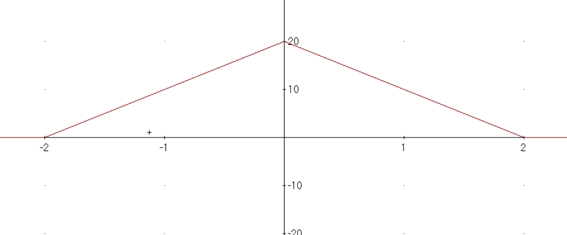
\includegraphics[scale=0.6]{Memoria/Aspectos_relevantes/Modificaciones_gravitatorias/Grafica_obstaculo_superdenso}
\caption{Gráfica que representa la influencia gravitatoria para una influencia máxima de 20, una influencia de 10 y un radio de región de influencia de 2 ($y = -10|X| + 20$)}
\end{figure}
\clearpage

Mientras se esté dentro de la región de influencia de un obstáculo superdenso se calculará el Vector2 que represente la influencia que ejerce sobre el KinematicObject y se añadirá a la lista de alteraciones de gravedad de la clase KinematicObjectGravityManager mediante el método AddGravityAlteration(Vector2).

\subsection{Inversor de gravedad}
Los inversores de gravedad invierten la gravedad del KinematicObject permanentemente al entrar en contacto con ellos. Para representar este proceso, se ha seguido una estructura de clases muy similar al patrón de diseño Observador. Hay una clase sujeto GravityInverterManager encargada de invertir la gravedad de los KinematicObjects y una clase observador GravityInverter encargada de decirle al sujeto que KinematicObjects tienen que invertir sus gravedades.

Cuando un observador detecta que un KinematicObject entra en contacto con él, le manda este KinematicObject al sujeto que comprueba si el KinematicObject está dentro de su lista y si no lo está lo añade. Si lo esta es removido de la lista.

En cada FixedUpdate el GravityInverterManager invierte la gravedad de todos los KinematicObject de la lista.

\begin{figure}[h]
\centering
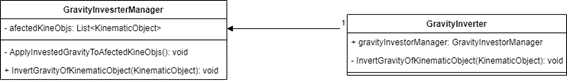
\includegraphics[scale=1]{Memoria/Aspectos_relevantes/Modificaciones_gravitatorias/Inversor_gravedad_UML}
\caption{Diagrama UML de la estructura del inversor de gravedad}
\end{figure}

\begin{figure}[h]
\centering
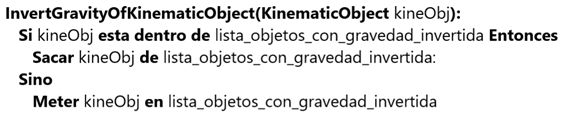
\includegraphics[scale=1]{Memoria/Aspectos_relevantes/Modificaciones_gravitatorias/Pseudocodigo_inversor_gravedad}
\caption{Pseudocódigo del método llamado cada vez que un KinematicObject entra en contacto con un inversor de gravedad}
\end{figure}

\begin{figure}[h]
\centering
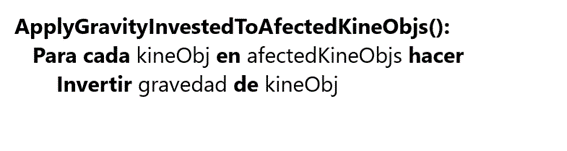
\includegraphics[scale=1]{Memoria/Aspectos_relevantes/Modificaciones_gravitatorias/Pseudocodigo_inverion_gravedad}
\caption{Pseudocódigo del proceso de inversión de gravedad de los KinematicObject en el FixedUpdate}
\end{figure}

Se ha creado un prefab que implementa el sistema de inversión gravitatoria llamado GravityInverterSystem que implementa todos los elementos necesarios para tener un sistema de inversión gravitatoria funcional.

\begin{figure}[h]
\centering
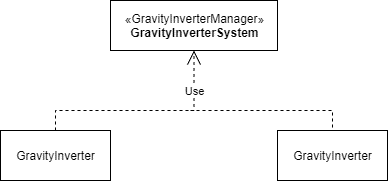
\includegraphics[scale=1]{Memoria/Aspectos_relevantes/Modificaciones_gravitatorias/GravityInverter_UML}
\caption{Estructura del prefab GravityInverterSystem}
\end{figure}

\section{Implementación de los obstáculos}
Los obstáculos son objetos que matan al Player al entrar en contacto con ellos. Hay tres tipos distintos de obstáculos: los obstáculos estáticos, los obstáculos que siguen una rutina y los obstáculos móviles.

\subsection{Obstáculos estáticos}
Los obstáculos estáticos son obstáculos que ocupan siempre la misma posición.

\begin{figure}[h]
\centering
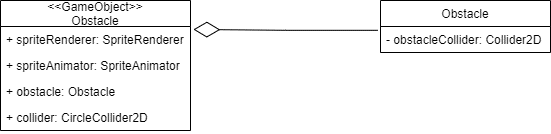
\includegraphics[scale=1]{Memoria/Aspectos_relevantes/Obstáculos/GameObject_obstaculo_estatico}
\caption{Estructura del GameObject asociado al obstáculo estático}
\end{figure}

Cuando una instancia de PlayerController entra en contacto con el Collider2D del obstáculo (Obstacle.obstacleCollider) se activa el evento PlayerObstacleCollision, que simplemente mata al Player y lo hace reaparecer en el punto de reaparición.

La estructura del obstáculo estático y la clase Obstacle son sencillas pero importantes, pues de ellas partirán el resto de obstáculos.

\begin{figure}[h]
\centering
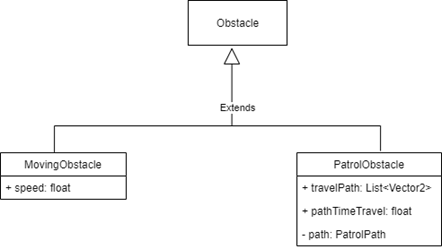
\includegraphics[scale=1]{Memoria/Aspectos_relevantes/Obstáculos/Herencia_obstaculos}
\caption{Jerarquía de herencia en la que el obstáculo móvil y el obstáculo que sigue una rutina heredan del obstáculo estático.}
\end{figure}

\subsection{Obstáculos que siguen una rutina}
Los obstáculos que siguen una rutina son un tipo especial de obstáculos que tienen una rutina definida. Esta rutina estará conformada por una lista de puntos en el mapa. El obstáculo irá desde un punto al siguiente de la lista haciendo una recta que sigue el camino más corto.\\
El obstáculo recorrerá en bucle esta rutina hasta que se salga o reinicie el nivel.

Se explica en profundidad el movimiento de los obstáculos que siguen una rutina en el anexo C.

\subsection{Obstáculos móviles}
Los obstáculos móviles son obstáculos que parten de un punto inicial y avanzan indefinidamente de izquierda a derecha a una velocidad establecida. La posición del obstáculo móvil en el frame actual se calcula añadiendo a la posición actual el vector dirección (Vector2.lef) por la velocidad establecida y por el tiempo entre frames (Time. fixedDeltaTime).

Esto se lleva a cabo mediante la instrucción ejecutada en cada FixedUpdate:

this.transform.position += (Vector3) Vector2.left * speed * Time.fixedDeltaTime;

\subsection{Clase ObstacleFabric}
Ante la necesidad de crear obstáculos móviles durante tiempo de ejecución se creó la clase ObstacleFabric. Esta clase es una aplicación del patrón de diseño Método Fabrica. ObstacleFabric tiene un método SpawnObject que devuelve una instancia del prefab establecido en la posición en la que se encuentra la fábrica.

De ObstacleFabric hereda una clase TriggerObstacleFabric que tiene asociada una clase PlayerTrigger. La clase PlayerTrigger es una clase que tiene asociado un Collider2D. PlayerTrigger tiene un atributo booleano isTrigger y mientras una instancia de PlayerController este en contacto con el collider de PlayerTrigger isTrigger será true y el resto del tiempo a false.

Cuando el Player entre en la zona de activación de PlayerTrigger (delimitada por el collider), TriggerObstacleFabric creará una instancia del prefab.

\begin{figure}[h]
\centering
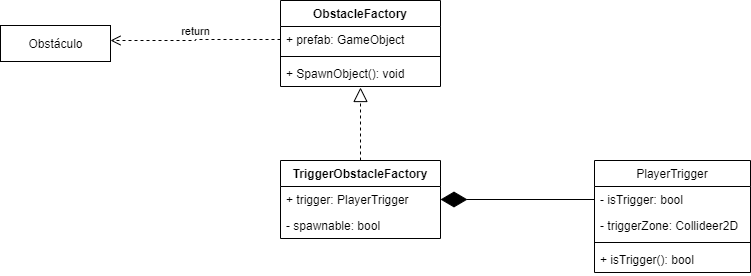
\includegraphics[scale=0.8]{Memoria/Aspectos_relevantes/Obstáculos/ObstacleFabric_UML}
\caption{Diagrama UML de la estructura de las fábricas de obstáculos}
\end{figure}

La intención de ObstacleFabric era que solo pudiese instanciar obstáculos, pero al elegir el obstáculo que se desea instanciar mediante la elección de un prefab lo que se pasa a instanciar es un GameObject y no un obstáculo, haciendo que aunque la fábrica se utilice exclusivamente para instanciar obstáculos, realmente se puede instanciar cualquier GameObject.

\subsection{Clase ObstacleDestroyer}
Los obstáculos móviles tienen una vida útil muy corta pues solo son necesarios desde que aparecen hasta que han atravesado toda la pantalla. Sin embargo cuando han perdido utilidad siguen desplazándose hacia la derecha consumiendo recursos de manera similar a como lo haría un proceso zombie. Para evitar esto se ha creado una clase ObstacleDetroyer que tiene asociado un Collider2D. Cuando los obstáculos entran en contacto con el collider del ObstacleDestroyer, el obstáculo se destruye liberando los recursos ocupados en él.

\section{Implementcación de los portales}
Los portales son GameObject organizados por parejas que permiten convertir la posición de un KinematicObject que entra a un portal en la posición del portal parejo al portal de aquel por el que se ha entrado (simulando la teletransportación entre portales).\\
Es una clase muy sencilla. La única complejidad reside en desactivar los portales durante el proceso de teletransportación para evitar que el KinematicObject se quede enganchado teletransportándose infinitamente de un portal a otro; y reactivarlos al salir del portal.

\begin{figure}[h]
\centering
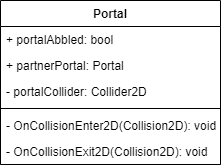
\includegraphics[scale=1]{Memoria/Aspectos_relevantes/Portales/Portales_UML}
\caption{Diagrama UML de la clase Portal}
\end{figure}

Como se ha mencionado anteriormente, los Portales se organizan en parejas. Se ha creado un prefab PortalCouple que es un GameObject con un par de portales asociados entre sí.

\begin{figure}[h]
\centering
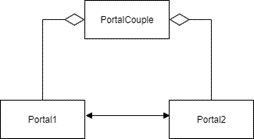
\includegraphics[scale=1]{Memoria/Aspectos_relevantes/Portales/Couple_portals}
\caption{Estructura de relaciones del GameObject PortalCouple}
\end{figure}

\section{Creadores de impulso}

Los creadores de impulso son objetos que aplican una variación en la velocidad que llevan a los objetos kinemáticos que entran en contacto con ellos. Hay tres tipos de creadores de impulso: la plataforma de salto, la partícula de impulso y el amplificador de impulso.
Para los creadores de impulso se ha decidido aplicar el patrón de diseño Puente.
\clearpage

\begin{figure}[h]
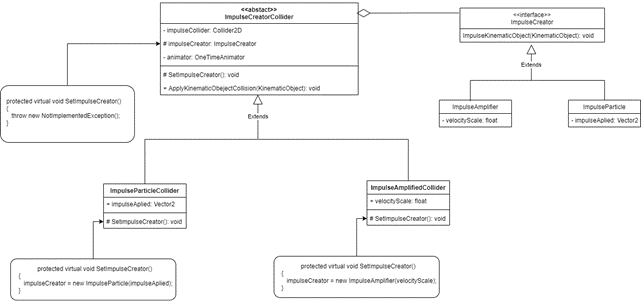
\includegraphics[scale=0.8]{Memoria/Aspectos_relevantes/Creadores_impulso/Creadores_impulso_UML}
\caption{Estructura de relaciones del GameObject PortalCouple}
\end{figure}

No se he decidido aplicar el patrón Puente porque el funcionamiento de los creadores de impulso valla a cambiar en tiempo de ejecución (que no lo hace), sino para reforzar la separación ente las clases encargadas de detectar las colisiones y las clases encargadas de aplicar el impulso evitando un vínculo permanente entre estas dos jerarquías de clases que haga más engorroso el proceso de adición o modificación de clases en una de las dos jerarquías establecidas.

\subsection{Sistema de gestión de las colisiones con los creadores de impulso}
Las colisiones de los creadores de impulso con los KinematicObject se han implementado siguiendo el mismo modelo que la colisión con los “Wall” (paredes y muros). La clase KinematicObjectCollisionManager llama al método BoxCastAll en la posición en la que se va a encontrar el KinematicObject en el siguiente frame. Si va a haber colisión con un creador de impulso se invoca al método ApplyKinematicObjectCollision del ImpulseCreatorCollider que delega la labor de aplicar el impulso a la instancia de ImpulseCreator que tiene asociada.\\
Explicado a grandes rasgos KinematicObjectCollisionManager avisa a ImpulseCreatorCollider de que se va a producir una colisión y este ordena a ImpulseCreator que aplique el impulso correspondiente al KinematicObject asociado al KinematicObjectCollisionManager.

\subsection{Tipos de creadores de impulso}
\subsubsection{Partícula de impulso}
Objeto que aplica un impulso en la dirección marcada por un Vector2 (ImpulseParticle.impulseAplied).

\begin{figure}[h]
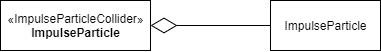
\includegraphics[scale=0.8]{Memoria/Aspectos_relevantes/Creadores_impulso/Particula_impulso}
\caption{Estructura del prefab asociado a la partícula de impulso}
\end{figure}

\subsubsection{Plataforma de salto}
Objeto similar a la partícula de impulso pero con la excepción de que el impulso aplicado solo puede ser en el eje vertical (ImpulseParticle.impulseAplied.X será siempre 0).

\begin{figure}[h]
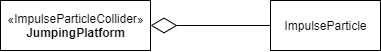
\includegraphics[scale=0.8]{Memoria/Aspectos_relevantes/Creadores_impulso/Plataforma_salto}
\caption{Estructura del prefab asociado a la plataforma de impulso}
\end{figure}

\subsubsection{Amplificador de impulso}
Objeto similar a la partícula de impulso, solo que en vez de añadir un impulso escala la velocidad que lleva el objeto kinemático con el que colisionag. La velocidad se escala ImpulseAmplifier.velocityScale veces.

\begin{figure}[h]
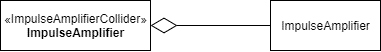
\includegraphics[scale=0.8]{Memoria/Aspectos_relevantes/Creadores_impulso/Amplificador_impulso}
\caption{Estructura del prefab asociado al amplificador de impulso}
\end{figure}

\section{Animación de los sprites}
Salvo para el Player, que se ha utilizado un animator de Unity, para el resto de objetos que requerían de un proceso de animación ha sido necesaria la creación de clases encargadas de la animación de estos objetos.\\

\begin{figure}[h]
Las clases encargadas de la animación son SpriteAnimator y OneTimeAnimator.

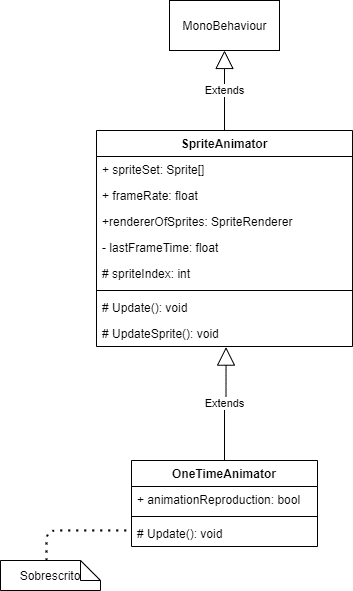
\includegraphics[scale=0.8]{Memoria/Aspectos_relevantes/Animadores/Herencia_animators}
\caption{Estructura de herencia de los animadores de sprites}
\end{figure}

Ambos animadores de sprites se encargan de reproducir una animación marcada por un vector de Sprite dado (SpriteAnimator.spriteSet). La diferencia entre las dos clases es que SpriteAnimator reproduce la animación en bucle indefinidamente (si llega al último Sprite del vector, el siguiente será el primero del vector), mientras que OneTimeAnimator reproducirá la animación una sola vez (cuando la variable OneTimeAnimator. animationReproduction sea true).

\subsection{UpdateSprite()}
El método UpdateSprite es el encargado de generar el efecto de reproducción de una animación mediante su llamada en cada Update. UpdateSprite cambia el Sprite a renderizar por el SpriteRenderer del GameObject cada $\frac{1}{SpriteAnimator.frameRate}$ segundos.

 
Esta división surge de que SpriteAnimator.frameRate lleva la cuenta de cuantos Sprites se tienen que reproducir en un segundo, con lo que cada $\frac{1}{SpriteAnimator.frameRate}$ se actualizará el Sprite a renderizar.

Para saber si hay que pasar a renderizar el siguiente Sprite se consulta la variable SpriteAnimator.lastFrameTime, que guarda el momento de tiempo en el que se actualizó por última vez el Sprite del SpriteRenderer. Cuando la diferencia entre Time.time (variable float que cronometra cuanto tiempo de ejecución lleva el programa) y SpriteAnimator.lastFrameTime sea mayor que $\frac{1}{SpriteAnimator.frameRate}$ (el tiempo transcurrido entre actualizaciones de Sprites) se actualizará el Sprite a renderizar y se recalculará SpriteAnimator.lastFrameTime.

\begin{figure}[h]
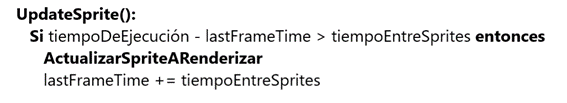
\includegraphics[scale=1]{Memoria/Aspectos_relevantes/Animadores/Pseudocodigo_UpdateSprite}
\caption{Pseudocódigo de UpdateSprite}
\end{figure}

\section{Clase GameController y estado de juego estable}
Se ha desarrollado una arquitectura específica para asegurar que los niveles jugables tienen están siempre en un estado estable de juego, y un proceso a seguir cada vez que se reinicia el nivel a su estado inicial.\\
Con este propósito se ha creado la clase GameController. El funcionamiento de esta clase se explica en profundidad en el anexo C.

\begin{figure}[h]
\centering
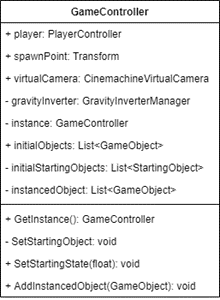
\includegraphics[scale=1]{Memoria/Aspectos_relevantes/GameController/GameController}
\caption{Diagrama UML de la clase GameController}
\end{figure}

Esta clase contiene dos elementos distintos al servicio del mismo propósito

\subsection{Variables de PlatformerModel}
La clase GameController contendrá una serie de atributos que, al iniciar la escena copiará en la clase PlatformerModel esos atributos. Estas variables son variables relevantes del nivel. Son movidas a la clase PlatformerModel para que todos los objetos de la escena puedan acceder a estas variables facilmente sin generar cadenas de mensajes para tener acceso a ellas.

Las variables de GameController que serán copiadas a PlatformerModel serán:
\begin{itemize}
\item
La CinemachineVirtualCamera que utiliza la escena (PlatformerModel.virtualCamera).
\item
El PlayerController asignado al avatar jugable (PlatformerModel.player).
\item
El objeto de tipo Transform asociado al punto de reaparición e inicio de escena del Player (PlatformerModel.spawnPoint).
\item
El GameController de la escena (PlatformerModel.gameController).
\item
El GravityInverterManager asociado a la escena \\ (PlatformerModel.gravityInverterManager).
\end{itemize}

\subsection{Estado inicial de juego}
Cuando el Player muera será necesario devolver el nivel al estado inicial en el que se encontraba al acceder a esa escena.\\
Para volver a este estado inicial será necesario:
\begin{itemize}
\item
Eliminar los objetos creados que no estaban instanciados al inicio del nivel.
\item
Devolver los objetos cuyo estado haya variado durante la ejecución del nivel a su estado inicial (un ejemplo sería devolver un obstáculo que sigue una rutina del punto en el que se encuentra al punto en el que empieza el juego).
\item
Instanciar objetos que estaban al inicio del nivel pero que ya no están instanciados.
\item
Devolver el Player a su posición inicial.
\end{itemize}

En la implementación del programa, se han tratado todos los objetos que debían ser devueltos a su estado inicial (salvo al Player) como el mismo tipo de objetos. Han sido guardados en una clase envoltorio que guarda el estado inicial del objeto. Estos objetos no serán los que estén en la escena, sino que en el estado inicial del juego se generarán clones de él en la escena.\\
Todos los objetos instanciados serán guardados en la lista instancedObjects para poder destruirlos cuando haya que reiniciar el nivel. Los objetos que se instancien durante la escena también serán añadidos a isntancedObjects.

\section{Mecánicas de tiempo bala}
Se han implementado una serie de mecánicas encargadas de escalar la velocidad a la que pasa el tiempo y como esto afecta a los objetos en la escena. Hay dos mecánicas de tiempo bala: escalar el tiempo a nivel global y escalar el tiempo de los objetos dentro de una zona. De los dos escalados de tiempo se encarga la clase TimeManager.

\clearpage
\begin{figure}[h]
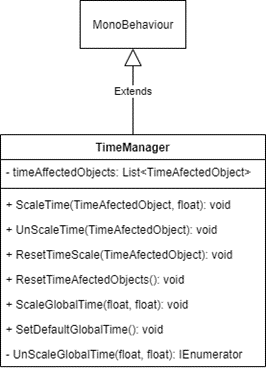
\includegraphics[scale=1]{Memoria/Aspectos_relevantes/Tiempo_bala/TimeManager_UML}
\caption{Diagrama UML de la clase TimeManager}
\end{figure}

\subsection{Escalado de tiempo global}
Es escalado de tiempo global es muy sencillo, pues Unity ya ofrece una herramienta que modifica el tiempo de todos los objetos. Se trata de la variable Time.scaleTime y todos los objetos relacionados con Unity se ven afectados por esta variable, incluidos los eventos (no los de la clase Simulation sino los propios de Unity).

A grandes rasgos Time.timeScale funciona multiplicando su valor por el “tiempo que tardará en llevarse a cabo la acción”. Siendo que si se tarda en ir de un punto ‘A’ a uno ‘B’ en X tiempo, se tardará en verdad X*Time.timeScale unidades de tiempo.

Del escalado del tiempo para todos los objetos se encargan las funciones TimeManager.ScaleGlobalTime, TimeManager.UnScaleGlobalTime y TimeManager.SetDefaultGlobalTime.

El escalado de tiempo global se aplica en la mecánica de tiempo bala del Player, escalando el tiempo y desescalandolo al los X segundos; y se aplica también en el estado estable del GameController (GameController.SetStartingState()).

\subsection{Zonas de escalado de tiempo}
Las zonas de tiempo escalado son objetos con un Collider2D. Cuando entre un TimeAfectedObject en el Collider2D, la zona de tiempo escalado escalará su tiempo hasta que salga de él.

\begin{figure}[h]
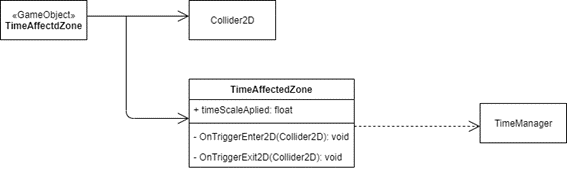
\includegraphics[scale=1]{Memoria/Aspectos_relevantes/Tiempo_bala/GameObject_zona_tiempo_escalado}
\caption{Estructura del GameObject asociado a las zonas de tiempo escalado}
\end{figure}

TimeAfectedObject es una clase abstracta de la que heredan los objetos que van a ser afectadas por las zonas de escalado de tiempo. TimeAfectedObject tiene el método abstracto Move, que es el que implementarán las clases con la intención de modificar el movimiento del objeto para adecuarse a la escala de tiempo que le ha sido aplicada.\\
Las zonas de escalado de tiempo imponen su escalado de tiempo a través de la clase TimeManager. Esto se debe a que TimeManager asume la responsabilidad de resetear el escalado de tiempo de todos los TimeAfectedObject. Esta necesidad surge de asegurar que en el estado de juego estable del GameController no haya TimeAfectedObject con el tiempo escalado. Es por ello que TimeManager tiene una lista de TimeAfectedObject en la que estarán todos los TimeAfectedObject cuyo tiempo haya sido escalado.

Se profundiza en la estructura de los TimeAffectedObject en el anexo C.

\section{Menús de los juegos}
Se ha desarrollado un sistema de menús de juego y transiciones entre escenas.

\begin{figure}[h]
\includegraphics[scale=1]{Memoria/Aspectos_relevantes/Menus/Transición_entre_menus}
\caption{Diagrama de viaje entre los distintos menús y escenas}
\end{figure}

La escena de la que se parte es la escena de selección de nivel. De esta escena se puede cerrar la aplicación (botón “Exit”), pasar a la escena de menú de opciones y jugar el nivel que se escoja.
En el nivel jugable se puede abrir un menú de pausa que detiene la ejecución del nivel jugable hasta que se cierre el menú de pausa.
Lo que se puede hacer en el menú de pausa y en el menú de opciones es básicamente lo mismo. Sin embargo, son objetos distintos (uno es un canvas y otro es una escena) con navegación a escenas distintas. Adicionalmente, el menú de pausa tiene la tarea añadida de parar la ejecución de la escena. Es por esto que se han tratado y desarrollado como elementos distintos.

\subsection{Menú de pausa}
El menú de pausa es un objeto con dos elementos fundamentales: la clase OptionsCanvasManager y un objeto hijo del menú de pausa que es un Panel.

\clearpage
\begin{figure}[h]
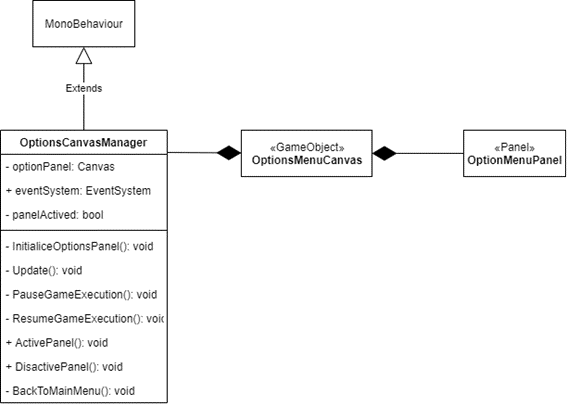
\includegraphics[scale=1]{Memoria/Aspectos_relevantes/Menus/GameObject_menu_pausa}
\caption{Diagrama de la estructura de GameObject asociado al menú de pausa}
\end{figure}

OptionsCanvasManager se encarga de abrir y cerrar el menú al pulsar el botón correspondiente y pausar y retomar la ejecución de la escena respetivamente (OptionsCanvasManager.PauseGameExecution y OptionsCanvasManager.ResumeGameExecution).

Lo que se hace en verdad al abrir y cerrar el menú de pausa es activar y desactivar el Panel (que muestra la interfaz del menú de pausa) y el EventSystem (se explicará en el siguiente apartado).

\begin{figure}[h]
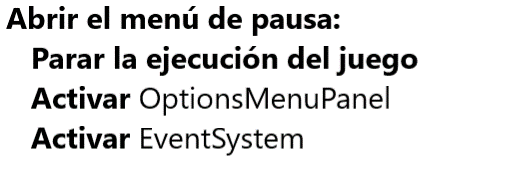
\includegraphics[scale=1]{Memoria/Aspectos_relevantes/Menus/Pseudocodigo_abrir_menu_pausa}
\caption{Pseudocódigo de las operaciones llevadas a cabo al abrir el menú de pausa}
\end{figure}

\begin{figure}[h]
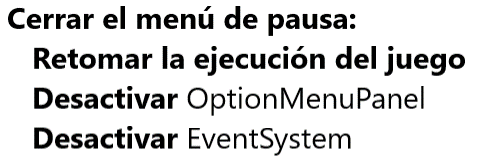
\includegraphics[scale=1]{Memoria/Aspectos_relevantes/Menus/Pseudocodigo_cerrar_menu_pausa}
\caption{Pseudocódigo de la operaciones llevadas a cabo al cerrar el menú de pausa}
\end{figure}

\subsection{Método de selección de elementos UI}
Para navegar entre los elementos del menú de utiliza un objeto de la clase EventSystem. Este objeto se encarga de manejar eventos de Unity (que no tienen nada que ver con los eventos de Simulation). Este objeto se utiliza para captar los botones de navegación pulsados y navegar al elemento UI correspondiente. Es por esto que al abrir y cerrar el menú de opciones también se activa y desactiva el EventSystem. Si no se desactiva el EventSystem los elementos del menú de opciones variarán en función de los botones pulsado a pesar de estar cerrado (por ejemplo modificando el volumen del juego sin abrir el menú de opciones). 

\subsection{Patrón de colores utilizados}
El patrón de colores utilizado para los elementos UI es el siguiente:

\clearpage
\begin{figure}[h]
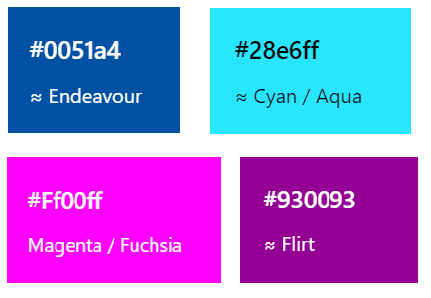
\includegraphics[scale=1]{Memoria/Aspectos_relevantes/Menus/Patron_colores}
\caption{Patrón de colores utilizado para la UI}
\end{figure}

\section{Sistema de modificación de volumen persistente}
En las opciones hay dos opciones: una que permite variar el volumen general del juego y otra que permite variar el volumen de las canciones que suenan. La idea es que cambiar el volumen haga este cambio persistente, manteniéndose entre escenas y ejecuciones del programa. Para ello han sido necesarias dos clases: VolumeManager y AudioSourceVolumeManager.

VolumeManager es una clase estática encargada de consultar y modificar el valor persistente de ambos tipos volumen. Este valor corresponde con el valor del volumen del juego que se encargará de leer y modificar VolumeManager y de compartirlo con las instancias de AudioSourceVolumeManager cuando lo requieran. Esto se hace mediante la clase PlayerPrefs, clase que ofrece Unity para guardar el valor de variables entre ejecuciones. Esto también se podría haber hecho guardando en un fichero los valores que se quiera que sean persistentes (que es lo que hace la clase PlayerPrefs al final), pero siendo que solo se desea almacenar el valor de variables se ha optado por la solución más simple. Si se hubiese querido se habría podido utilizar un fichero, pero hay que guardarlo en la ruta ofrecida por la variable Application.persistentDatatPath si se quiere que al exportar la aplicación se guarde y consulte correctamente el fichero.

La clase AudioSourceVolumeManager actúa como envoltorio del objeto AudioSource de Unity (el que se usa para reproducir audios). El volumen del AudioSource no se modifica explícitamente, sino que AudioSourceVolumeManager consulta el valor general del volumen en AudioSourceManager y se lo asigna al AudioSource del que tiene referencia. AudioSourceVolumeManager tiene una clase hija que es AudioSourceMusicVolumeManager, que modifica el volumen del AudioSource en función del volumen de la música además del volumen general.

\begin{figure}[h]
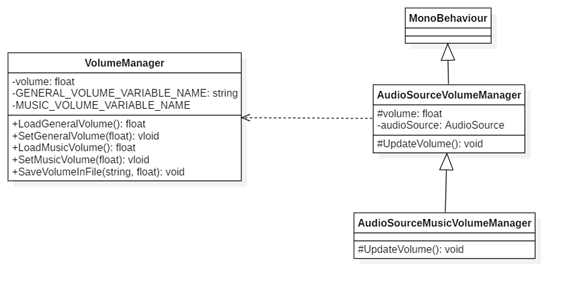
\includegraphics[scale=1]{Memoria/Aspectos_relevantes/Volumen_persistente/VolumeManager_UML}
\caption{Diagrama UML que representa la relación entre VolumeManager y AudioSourceVolumeManager}
\end{figure}

\subsection{Escenas que comparten canción}
Las escenas GameMenu y OptionsScene comparten canción, de manera que aunque se cambien entre estas dos escenas la canción que suena no dejará de reproducirse. En verdad sí que lo hará, pero lo que sucede es que al viajar entre estas escenas se guardará (en una variable estática) el segundo de la canción que se está reproduciendo y al entrar a la otra escena se reproducirá la canción pero continuando desde el punto en el que había dejado la canción la escena anterior. Cuando desde estas dos escena se viaje a una que no es esa, en vez de guardar el segundo de la canción en el que se está, se reseteará la variable donde se está guardando el segundo de la canción (poniéndolo a 0) y haciendo así que la próxima vez que se entre a estas escenas la canción se empiece a reproducir de cero.

\subsection{Clase VolumeSliderBar}
El volumen general se modifica en la clase VolumeSliderBar, que tiene asociado un elemento UI Slider. VolumeSliderBar consulta el valor del Slider y se lo asigna al volumen de VolumeManager. VolumeSliderBar es una clase abstracta con dos hijos: GeneralVolumeSliderBar para modificar el volumen general y MusicVolumeSliderBar para el volumen de las canciones que suenan.

\section{Desarrollo de la gestión de la cámara}
Se va a documentar en la memoria el proceso de desarrollo de la gestión de la cámara a la vez que se desarrolla, pues se considera un muy buen ejemplo de desarrollo de uno de los elementos de un videojuego y suficientemente representativo como para entender el proceso. Además va a resultar interesante, pues se va a razonar el funcionamiento de las cámaras y las decisiones que se han tomado para escoger un funcionamiento de la cámara y no otro.

La mayoría de la información obtenida para la toma de decisiones durante este proceso ha sido obtenida de la siguiente URL de la página de Gamasutra \cite{Gamasutra}:\\
 \url{https://www.gamasutra.com/blogs/ItayKeren/20150511/243083/Scroll_Back_The_Theory_and_Practice_of_Cameras_in_SideScrollers.php}.
 
Este enlace contiene otro enlace a una charla en la que se explican estos conceptos en video.

\subsection{Introducción al sistema gestor de cámaras}
La cámara va a ser el elemento encargado de mostrar por pantalla la región del espacio del nivel que se desea mostrar. El principal conflicto que afecta a la cámara es que en distintos momentos del juego se quiere mostrar espacios distintos del escenario. Por suerte este problema es más sencillo de lo que parece en un principio, pues la mayoría del rato las distintas regiones del espacio que se deseen mostrar estarán condicionados por un elemento principal que se mueven en el espacio (en el caso de este juego y la mayoría, ese elemento será el avatar que utilice el jugador). Ese problema tiene una solución relativamente sencilla y, sobre todo explorada por juego hechos en el pasado, que es hacer que la cámara siga a ese elemento principal.

En este videojuego, afortunadamente, el único elemento principal que hay que seguir es el jugador. En otros videojuegos esta tarea puede ser más compleja, ya sea debido a que cambia el objetivo principal (a un elemento que hay que perseguir o una pantalla que avanza con el tiempo por ejemplo) o que hay varios objetivos principales (como en un juego multijugador local o en una batalla contra un jefe, donde los objetivos principales son tanto el jugador, como el jefe).

Sin embargo, aunque solo haya un objetivo principal en el juego (el jugador), puede ser que en el haya objetivos secundarios que no merezcan que la cámara los siga específicamente a ellos, pero sí tenerlos en cuenta. En lo que se lleva de desarrollo hasta ahora hay dos objetivos secundarios que generan conflicto: los portales y los obstáculos. Estos objetivos secundarios son variados y generan conflictos distintos sobre la cámara. Se van a explicar a continuación.

\subsection{Conflictos con los portales}
Los portales son los elementos que más dudas me generan acerca de cómo afrontarlos. El problema de los portales es que trabajan en parejas. Al entrar por un portal, sales por el portal pareja de este, independientemente de si está en el rango de lo que permite ver la cámara. Con el sistema de gestión de cámaras que ofrece Plataformer Microgame (el usado hasta ahora) la cámara apunta exactamente al punto donde está el jugador. Esto para los portales resulta bastante conveniente, pues según el jugador atraviesa el portal la cámara sigue apuntando a la posición del jugador, dando visión instantáneamente del jugador dificultar la visión de lo que el jugador tiene ahora en su nuevo entorno. En términos de ofrecer visión al jugador es una solución bastante eficaz, pero adolece de un gran problema: el jugador ahora no sabe dónde está. El jugador ahora se haya desorientado. El jugador anteriormente tenía una referencia clara de donde se encontraba (básicamente se había a la derecha del punto de inicio), pero ahora no tiene ni idea de donde está ni adonde tiene que ir. La escena de prueba de los portales es una muy buena práctica para comprobar si el diseño de los portales desorienta o no.

\clearpage
\begin{figure}[h]
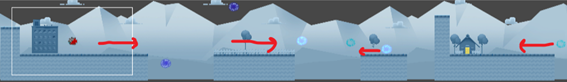
\includegraphics[scale=1]{Memoria/Aspectos_relevantes/Camaras/PruebaPortalScene}
\caption{Escena PruebaPortalScene}
\end{figure}

En la imagen se ha dibujado flecha en cada plataforma con el sentido que se espera que siga el jugador para llegar hasta la zona de victoria. En esta escena el jugador no solo no puede ver los dos portales que forman una pareja de portales y deducir por donde de donde ha venido, sino que además se está cambiando continuamente la dirección que se espera que tome el jugador tome. Un jugador probablemente no sea capaz de deducir que camino ha de tomar de manera intuitiva.

Una solución parcial a este problema podría ser al principio del nivel mostrar el nivel entero e ir haciendo Zoom-in hasta llegar al jugador y dejar la cámara en la posición que tendrá por defecto. Pero esto no es solo un parche improvisado al problema, sino que además en niveles grandes habrá demasiados elementos como para que ese recurso permita ver nada y mucho menos permitir al jugador deducir el camino que debe seguir.\\
Este problema no desaparece con este sistema de gestión de cámaras y se ha de tener en cuenta en el nuevo que se va a implementar.

El segundo problema que provocan los portales es una premonición del sistema que probablemente se acabe implementando. Se pretende que la cámara siga al jugador, no que apunte estrictamente a él. Con los portales surge el problema de que, al mover al jugador a una posición alejada del punto en el que se encontraba un frame antes, la cámara ahora se tiene que mover hasta ahí pudiendo hacer que en lo que llega la cámara ocurra algo que el jugador no haya visto. Reduces “innecesariamente” la información que el jugador puede obtener a través de la cámara. El problema de orientación del jugador que se soluciona con el sistema de cámara que se planea implementar se sustituye por este. Este problema se pude solucionar haciendo que no suceda nada en las cercanías de los portales pero a costa de limitar la creatividad y variedad que los portales ofrecen al salir de uno.

\subsection{Conflictos con los obstáculos}
Aquí el problema es solo uno: Puede ser que el tiempo de reacción ante la aparición de un obstáculo y el espacio que la cámara ofrece para que el jugador se dé cuenta de que está en riesgo de colisionar con un obstáculo sean demasiado pequeños. Este problema se va a separar en tres tipos de obstáculos y como estos manifiestan el problema recién explicado.

\textbf{Obstáculos estáticos:} Los obstáculos que probablemente menos conflictos generen son los obstáculos estáticos. En principio casi cualquier tamaño de cámara permitiría ver y reaccionar ante este obstáculo. Pero en el juego que se está desarrollando no se va a tener en todo claro que velocidad va a llevar el jugador y es posible que algún obstáculo se haga excesivamente difícil de esquivar solo por el un mal implementado sistema de gestión de la cámara. Unity adicionalmente puede provocar confusión al respecto, ya que las distancias pueden llegar a percibirse distintas en el editor que en la pantalla de juego.\\
Por ejemplo la escena PruebaPlayerScene en el editor da la impresión de haber suficiente distancia entre el jugador y el obstáculo, pero en la pantalla de juego se ve como la distancia es menor y dependiendo de la velocidad con la que el jugador llegue puede ser que el jugador no tenga suficiente tiempo de respuesta como para esquivar el obstáculo.

\begin{figure}[h]
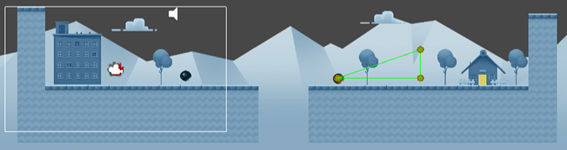
\includegraphics[scale=1]{Memoria/Aspectos_relevantes/Camaras/PruebaPlayerScene}
\caption{Escena PruebaPlayerScene}
\end{figure}

\clearpage
\begin{figure}[h]
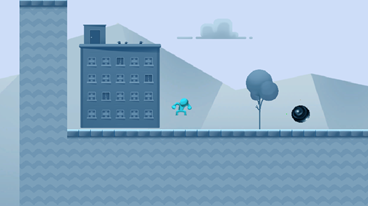
\includegraphics[scale=1]{Memoria/Aspectos_relevantes/Camaras/Camara_PruebaPlayerScene}
\caption{Visión de la escena PruebaPlayerScene desde la cámara.}
\end{figure}

\textbf{Obstáculos que siguen patrones:} Con los obstáculos que siguen patrones el problema evidente reside en que al salir del cámara el jugador no tiene conocimiento de por dónde va a volver a entrar en cámara. Aquí el problema reside en como decidir si intentar incluir el obstáculo en la cámara o no.
La posición del obstáculo que sigue un patrón está determinada por el patrón de movimiento que sigue y este puede ser muy variado y recorrer un gran espacio del nivel, haciendo un difícil deducir si la cámara debe centrarse en incluir el obstáculo en la cámara o no.

\textbf{Obstáculos móviles:} Estos son los obstáculos más problemáticos (sobre todo los obstáculos móviles veloces) pues van de un extremo al otro de la cámara y no hay forma de saber cuándo hay un obstáculo y cuando no. Hay herramientas que pueden facilitar saber si uno de esos obstáculos se acercan o no al jugador como, por ejemplo, utilizar sonidos que identifiquen si hay un obstáculo móvil o no y jugar con el volumen de este sonido para que el jugador pueda intuir la distancia a la que se encuentra. Es cierto que estas medidas son más eficaces que un buen sistema gestor de cámaras. Pero uno de los objetivos del sistema gestor de cámaras es no resultar tan inconveniente como para que resulte imposible esquivar los obstáculos móviles.\\
Lo más probable es que este problema se solucione con que la cámara sea de un tamaño lo suficientemente grande como para ofrecer suficiente tiempo de respuesta permitiendo esquivar los obstáculos. Pero en caso de no ser suficiente igual es necesario hacer algún cambio sobre el sistema de gestión de cámaras para solucionar este posible problema.

\subsection{Sistema de gestión de cámaras que se va a utilizar}
La cámara va a constar de dos elementos: el controlador de la cámara y el objetivo de la cámara. El controlador de la cámara se encargará de mover la cámara a donde el objetivo de la cámara se encuentre. El objetivo de la cámara se encargará de hacer los cálculos necesarios para decirle a la cámara donde debe apuntar.\\
El controlador de la cámara es muy sencillo, pues solo es poner la posición en la misma posición que el objetivo. Lo interesante es el objetivo de la cámara, pues se van a tener en cuenta varias cosas para decidir donde se va a posicionar. La cámara, explicado brevemente, va a funcionar siguiendo el movimiento del jugador.\\
Inicialmente se planeó crear scripts que se encargasen de la gestión de las cámaras, pero resulta que existe un paquete para Unity que es el paquete “Cinemachine” \cite{PaqueteCinemachine}. Este paquete lo utiliza Plataformer Microgame y se ha obtenido conocimiento de él gracias a esta plantilla, que hace uso de una Cinemachine virtual camera. Teniendo en cuenta el tiempo que llevaría diseñar y desarrollar un sistema de gestión de cámaras a mano y la completitud y personalización de cámaras que ofrece este paquete se ha decidido hacer uso de él y adecuar el movimiento de la cámara al juego utilizando este paquete.

Este paquete ofrece un objeto que se llama Cinemachine virtual camera. Este objeto se aplica sobre un objeto de una escena añadiéndolo como un componente al GameObject asociado. Si le añades a una cámara el componente CinemachineBrain, esta cámara será la que pasará a actuar como objetivo de la cámara y el objeto con el componente Cinemachine virtual camera se comportará como el controlador de la cámara con el componente CincemachineBrain.\\
Una de las cosa que ofrece el objeto Cinemachine Virtual Camera es la capacidad de dividir el espacio que abarca la cámara en distintas regiones que afectaran de distinta forma al movimiento de la cámara. Los nombres que se le va a dar a estas zonas que se van a explicar a continuación son: la death zone, la soft zone y la hard zone. 

\clearpage
\begin{figure}[h]
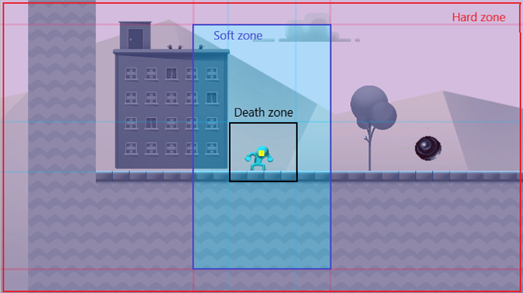
\includegraphics[scale=1]{Memoria/Aspectos_relevantes/Camaras/Camara_Cinemachine}
\caption{Distintas regiones que tiene en cuenta Cinemachine virtual camera.}
\end{figure}

A grandes rasgos Cinemachine virtual camera tiene en cuenta 4 cosas:
\begin{itemize}
\item
El objetivo a seguir (punto amarillo).
\item
La death zone (zona sin colorear).
\item
La soft zone (zona azul).
\item
La hard zone (zona roja).
\end{itemize}
El objetivo a seguir es el objetivo principal mencionado en la introducción. El objetivo principal es el objeto que se ha de mostrar en todo momento en cámara y que la Cinemachine virtual camera se encargará de mostrar por cámara siempre.\\
La death zone es la zona por la que se podrá mover el objetivo principal sin que la cámara se mueva. En cuanto el objetivo principal salga de la death zone la cámara se empezará a mover. El objetivo principal no es el objeto entero que se establece como objeto a seguir, sino el vector que representa su posición (se puede obtener mediante gameobject.transform.position), de manera que los límites del objeto pueden sí salirse de la death zone sin compromiso, pero solo mientras su posición que permanezca dentro de la death zone. Esto será así también para la soft zone y la hard zone.\\
Una vez el objetivo principal entre en la soft zone, la cámara comenzará a moverse hacia el objetivo principal hasta volver a meterlo en la death zone. La velocidad con la que la cámara persigue al objetivo principal depende de la distancia a la que este se encuentre (cuanto más lejos del centro de la cámara el objetivo principal, mayor será la velocidad de la cámara). El objetivo principal puede moverse por la soft zone sin que la cámara lo alcance mientras la cámara no tenga la velocidad necesaria para devolverlo a la death zone.
La hard zone es una zona por la que el objetivo principal no podrá desplazarse. En cuanto este alcance la hardzone, la cámara para devolver a la soft zone al objetivo principal. En realidad lo que hace la cámara es cambiar su posición a una en la que se encuentre el objetivo principal de la manera lo más consistente posible. Sinceramente, la Cinemachine virtual camera es bastante consistente a la hora de cambiar su posición a otra. Sin embargo, esta es la causa de uno de los dos problemas con los portales. Al cambiar la posición del objetivo principal a una que está en la hard zone, la cámara se mueve de una posición a otra sin hacer el recorrido que lleva de la posición anterior a la nueva, desorientando al jugador y haciendo que no sepa de donde ha venido.

Un sistema de gestión de cámara ideal sería uno que no posea hard zone, solo soft zone y death zone, de manera que al atravesar un portal la cámara también realice el recorrido de un portal a otro. A malas, este problema se puede solucionar haciendo que los portales no teletransporten al jugador de un punto a otro sino que simplemente lo muevan muy rápido. Esta puede ser una medida que se tome si no se logra aplicar el sistema gestor de cámaras deseado.

\subsection{Sistema de gestión de cámaras final}
El sistema de gestión de cámara que traía por defecto la plantilla de Platformer Microgame es la siguiente:

\clearpage
\begin{figure}[h]
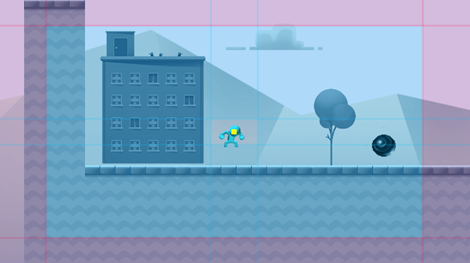
\includegraphics[scale=1]{Memoria/Aspectos_relevantes/Camaras/Cinemachine_Platformer_Microgame}
\caption{Sistema de gestión de cámaras de Platformer Microgames}
\end{figure}

Este sistema de cámaras tiene dos problemas principales: la vista de la cámara está demasiado cerca del personaje, dificultando al personaje ver lo que tiene alrededor y que dependiendo de la velocidad del jugador, es posible que la cámara no siga lo suficientemente rápido al jugador dificultando todavía más que el jugador tenga conocimiento de lo que tiene alrededor. El nuevo sistema de cámaras ha hecho dos cambios principales: alejar la visión de la cámara y reducir el rango de la soft zone. Alejar la visión se justifica por si sola. Reducir el rango de la soft zone permite que el avatar del jugador se encuentre siempre en el centro de la pantalla. De esta forma da igual la velocidad del jugador, que siempre se encontrará en el centro y contará con suficiente margen de pantalla para poder reaccionar a los elementos que surjan por los extremos de la pantalla.\\
Se han tomado otras dos decisiones adicionales. Una de ellas es aumentar la región ocupada por la death zone para que el jugador tenga una zona de estabilidad en la que no se mueve la cámara permitiéndole desplazarse con la estabilidad de que la cámara se mantenga estática y, adicionalmente, prepararle para el movimiento de la cámara, que no será tan brusco si el jugador ya se está moviendo frente a que la cámara empiece a moverse con el jugador.\\
La otra decisión ha sido desplazar la soft zone y la death zone un poco hacia la izquierda. Esta decisión se ha tomado con la intención de dar más espacio al jugador a ver lo que le viene desde la derecha. Esto se debe a que, en la mayoría de los casos, el lado izquierdo del mapa será conocido, mientras que el lado derecho es desconocido. Al tener conocimiento previo de lo que hay al lado izquierdo de la pantalla no hace falta tener visión absoluta del juego. Sin embargo, al encontrarse lo desconocido casi siempre en el lado derecho de la pantalla, se ha considerado recomendable mostrar más espacio al lado derecho de la pantalla que al izquierdo.

\begin{figure}[h]
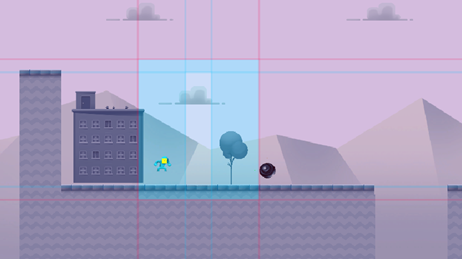
\includegraphics[scale=1]{Memoria/Aspectos_relevantes/Camaras/Camara_Cinemachine_juego}
\caption{Sistema de gestión de cámaras final aplicado}
\end{figure}

Ninguno de estos cambios solucionan el problema de los portales. Esto se debe a que, haciendo que la cámara siga la trayectoria entre portales, si los portales están a demasiada distancia (la principal razón para hacer que la cámara siga la trayectoria entre portales) el movimiento entre frames de la cámara es demasiado grande, desorientando al jugador más de lo que le ayuda a saber que camino ha recorrido. Se ha decidido solucionar este problema de otra forma, como por ejemplo dibujar líneas que conecten portales pareja.
\capitulo{6}{Trabajos relacionados}

\section{Juegos similares en género y mecánicas}
Este videojuego se inspira de otros dos videojuegos diferentes: Super Meat Boy \footnote{Enlace a la página de Wikipedia de Super Meat Boy: \url{https://es.wikipedia.org/wiki/Super_Meat_Boy}} y Celeste 
\footnote{Enlace a la página de Wikipedia de Celeste: \url{https://es.wikipedia.org/wiki/Celeste_(videojuego)}}. Esta temática es a nivel de género más que de mecánicas. Ambos juegos son plataformas 2D comprometidos con sus mecánicas y precisos en su jugabilidad. Es cierto que Celeste está más comprometida con la historia que Super Meat Boy, mientras este se centra casi exclusivamente en las mecánicas.

Celeste representa la variedad mecánica que se desea alcanzar, ofreciendo mecánicas distintas como acelerones y portales e incluso mecánicas que modifican el estado natural del juego (como permitir dar más de un acelerón en el aire cuando no se podría).

\clearpage
\begin{figure}[h]
\centering
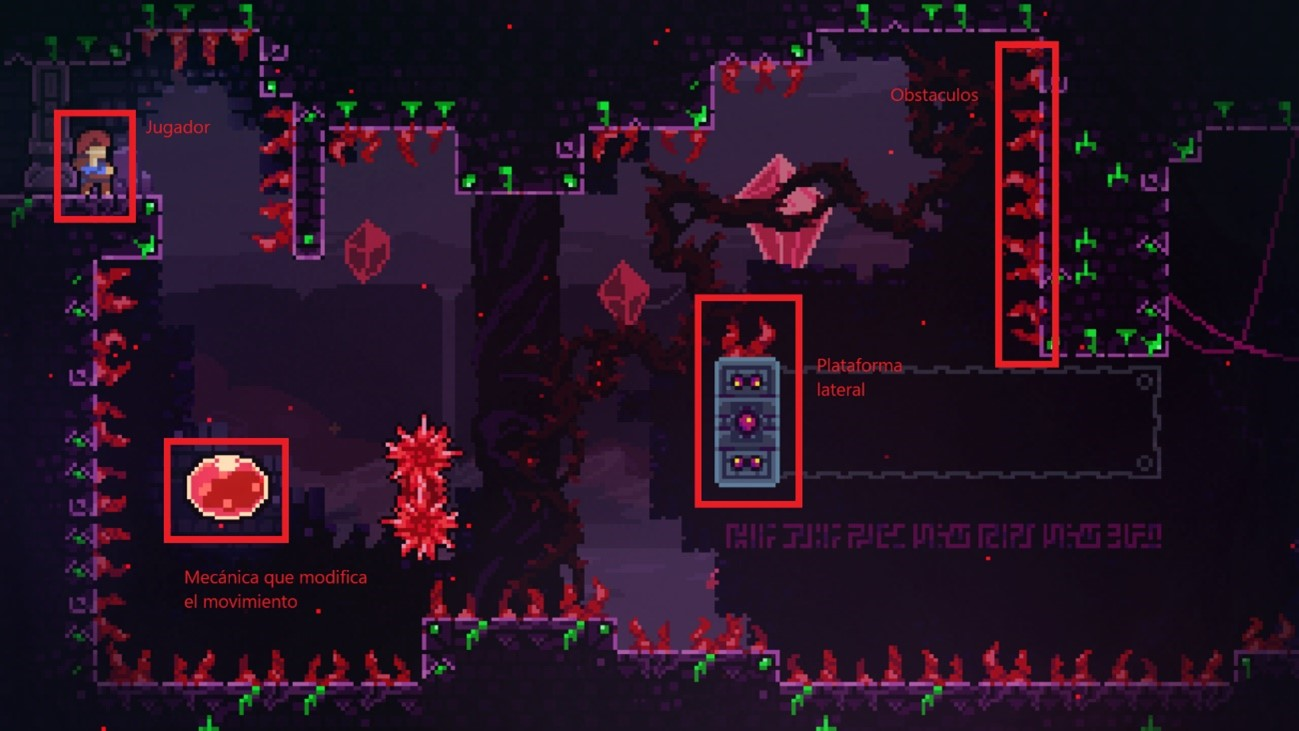
\includegraphics[scale=0.6]{Memoria/Trabajos_relacionados/Celeste}
\caption{Captura de pantalla de un nivel del videojuego Celeste.}
\end{figure}

El videojuego Super Meat Boy está muy concienciado con el movimiento del jugador. La calidad de este juego es tal, que el jugador es en todo momento consciente de donde está el avatar que controla y qué está haciendo. El juego le da mucha importancia a las físicas y como el jugador interactúa con ellas. Estas físicas no cambian, pero son un elemento muy bien establecido e intuitivo. En varios niveles el jugador tiene que hacer uso de las físicas y la inercia para superar obstáculos que en condiciones normales no sería capaz de superar.

\begin{figure}[h]
\centering
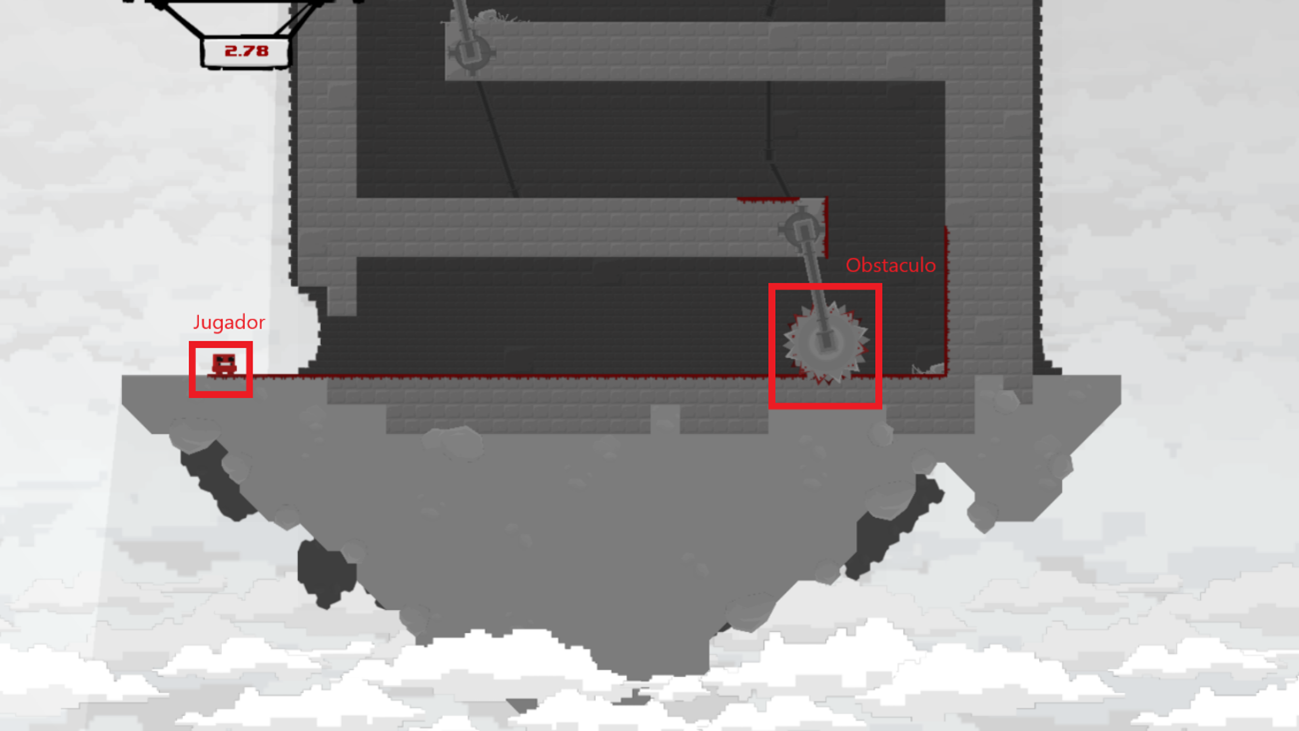
\includegraphics[scale=0.7]{Memoria/Trabajos_relacionados/Super_meat_boy}
\caption{Captura de pantalla de un nivel del videojuego Super Meat Boy.}
\end{figure}

En cuanto a la estructura de los niveles, Celeste y Super Meat Boy difieren ligeramente. En Celeste el nivel está dividido en subniveles que no tiene por qué ser independientes entre sí. El jugador escoge un capítulo y ese capítulo está dividido en una serie de niveles por los que el jugador viaja hasta alcanzar el último nivel y superar el capítulo. En la captura de pantalla anteriormente mostrada se puede observar cómo cada nivel de Celeste es cerrado, con unos límites definidos y una entrada y salida clara. El nivel generalmente se superará resolviendo un puzle que se manifiesta deduciendo un camino que requerirá el uso de distintas mecánicas para recorrerlo y llegar al siguiente nivel.

Los niveles de Super Meat Boy, como se puede observar en la captura de pantalla, no están limitados al alcance de la cámara, sino que la meta todavía no se ve. En el nivel mostrado en la captura se muestra un camino claro a seguir, pero no tiene por qué ser así.

A diferencia de Celeste, los niveles de Super Meat Boy son independientes entre sí y la salida de un nivel no es la entrada a otro, mas es cierto que se sigue una temática en la que los niveles siguen un patrón visual similar. 

Con el presente trabajo se desea seguir una estructura de niveles similar a Super Meat Boy, con niveles abiertos, independientes entre sí y que no están limitados a la visión de la cámara.
Para las mecánicas se va a seguir el ejemplo de Celeste, incluyendo mecánicas visuales y variadas que generen interacción entre sí.

La temática y mecánicas de modificación de las físicas y el tiempo es la parte original a implementar en el videojuego. Mencionar aun así, que se utilizan mecánicas que no son enteramente originales (como el tiempo bala que se utiliza en otros géneros y en algunos otros juegos de plataformas) pero que se van a adaptar al género de plataformas 2D.

Existe un juego de plataformas 2D que se llama Braid \footnote{Página de la Wikipedia de Braid: \url{https://es.wikipedia.org/wiki/Braid}} e implementa mecánicas de viajes en el tiempo. Sin embargo, este juego tiene una temática más seria y sus mecánicas de viaje en el tiempo están más enfocadas a la resolución de un puzzle que en el disfrute inherente a usarlas con maestría. Al tener una intención tan distinta no se considera un buen referente.

\section{Evaluación de Plataformer Microgame}
Para el desarrollo del videojuego se planteó partir de una plantilla de proyecto que proporcionase las bases del videojuego. Como plantilla de partida se eligió Plataformer Microgame \cite{PlatformerMicrogame} y se realizó un estudio de la platilla para ver si era válida como punto de partida. Del estudio se obtuvo un análisis de los elementos que ofrece Plataformer Microgame.

\begin{figure}[h]
\centering
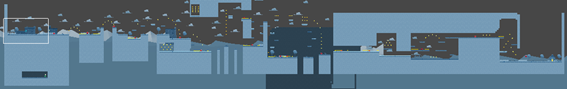
\includegraphics[scale=0.7]{Memoria/Trabajos_relacionados/Nivel_Platformer_Microgame}
\caption{Nivel de presentación de Platformer Microgame}
\end{figure}

\subsection{Grid}
Unity tiene un objeto que es el Tilemap. Este objeto permite de manera sencilla representar escenarios a partir de sprites añadidos al editor de Tilemaps. Grid es un objeto formado por una serie de Tilemaps (Foreground, Background, FarBackground y level) para formar el escenario de la escena del nivel.

\subsection{UI Canvas}
Ofrece una plantilla como punto de partida para la creación de elementos UI (User Interface).

\subsection{Enemies}
Objeto que agrupa todos los enemigos en un objeto para tenerlos centralizados y fácilmente alcanzables e identificables. En la plantilla de Platformer Microgame hay un tipo de enemigo implementado por defecto, que es el mostrado en la escena de muestra de la herramienta. Los enemigos pueden estar estáticos en un punto o seguir un patrón de movimiento.

\subsection{Tokens}
Son los típicos coleccionables de los juegos. Estos tokens tienen dos scripts que se encargan de ellos: uno para manejar las animaciones y otro para la colisión y recolección del coleccionable por parte del jugador.

\subsection{Zones}
Objeto encargado de agrupar todas las zonas de interés del nivel. Un ejemplo de estas zonas serían las zonas de victoria y de muerte del nivel (si el jugador toca la zona de victoria ganará y si toca la de muerte morirá).

\subsection{GameController}
Contiene los elementos necesarios para el funcionamiento del juego como conjunto. Principalmente contiene una clase con datos que las clases del nivel utilizaran, una clase encargada de animar los coleccionables (tokens) y una clase encargada de mostrar u ocultar el menú de pausa del juego.

\subsection{Player}
Objeto que representa el avatar que controlará el jugador.

\subsection{Simulation}
La clase Simulatión es una clase muy útil con una subclase Events. La clase Simulation tiene una cola en la que se encolarán eventos (clases que hereden de Simulation.Event). En cada frame se reproducirán todos los eventos encolados pendientes de ejecutarse.

Se explica en profundidad el funcionamiento de esta clase en el anexo C.

\subsection{Pegas}
Hay una serie de pegas importantes que se han encontrado en la plantilla de Plataformer Microgame y que han sido importantes a la hora de elegir si utilizarla o no.

\subsubsection{AnimationController}
AnimationController es la clase que implementas las físicas y la animación de los objetos (en la escena solo se aplica a los enemigos).
Esta clase se encarga de animar y controlar las físicas de los enemigos. Se viola el principio de responsabilidad única, además con dos mecánicas muy distintas como son las físicas y las animaciones. Debería separarse en dos clases distintas, una para la animación y otra para las físicas. Esto es importante porque, actualmente, en caso de querer variar las físicas o las animaciones de un enemigo tienes que reescribir todo el método ComputeVelocity() modificando tanto físicas como animaciones. El script PlayerController adolece de los mismos problemas. 
Adicionalmente delega a la animación el movimiento de todo el enemigo, lo cual obliga a las animaciones a encargarse del movimiento, tarea que no le corresponde.

\subsubsection{Health}
Health hereda de MonoBehaviour, pero no tiene necesidad de heredar de esta clase, ni heredar sus métodos y responsabilidades. La única función que sobrescribe de MonoBehaviour es Awake, función que puede ser perfectamente sustituida por un constructor. Adicionalmente, Health no tiene un método para devolver la salud a un estado inicial o por defecto, haciendo que tanto a la hora de restablecer la salud de un objeto como a la hora de restablecer la salud del Player cuando reaparece después de morir, se aplique el método Increment, método que no corresponde a esa acción.

\subsubsection{SpawnPoint}
SpawnPoint es un objeto de la escena supuestamente creado para determinar el punto de aparición del jugador, sin embargo esto solo se aplica cuando el jugador muere, de manera que inicia el juego en una posición y reaparece en otra. Esto hace muy improbable que el punto de reaparición sea el mismo que el punto en el que apareces al entrar a la escena, lo cual (en este tipo de juegos) no tiene sentido.

\subsubsection{JumpState}
La clase PlayerController maneja los estados de salto mediante una enumeración, manejándolos mediante un switch. Esto viola el principio Open/Close y centraliza todas las operaciones correspondientes a los estados en PlayerController agrandando la clase. 
En lo relativo a la acción de salto el atributo de deceleración (jumpDeceleration) del salto solo se aplica si no se mantiene el botón de salto pulsado hasta el fin de la acción de salto. Esto hace que el salto corto aplique la deceleración pero el salto largo no, de manera que la misma acción puede desenvolverse de dos formas distintas. 

\subsubsection{Rigidbody2D.Cast}
El Player utiliza el método Cast() de su Rigidbody2D para detectar los elementos que tiene a su alrededor y actuar en consecuencia. Esto provoca que todas las superficies con las que choca sean tratadas iguales, ya sean paredes o suelo, lo que desemboca en que el jugador al saltar mientras está al lado de una pared “colisione” con ella y cancele el salto a mitad de la acción. Adicionalmente puede ser un inconveniente utilizar este método a la hora de añadir mecánicas como trepar por las paredes o deslizarse por el suelo. 

\subsubsection{PatrolPath.Mover}
Los métodos establecen la forma de obtener la posición que ocupa el objeto en el momento, pero no hay límites explícitos que permitan saber por ejemplo si se ha terminado de ejecutar el movimiento o no. Esto no supone un problema debido a la implementación del código, pero, sería preferible establecer unos límites convirtiendo la clase en algo similar a un iterador, que en cada paso calcule la siguiente posición del objeto.

\subsection{Conclusiones}
La clase Simulation es la base del funcionamiento del juego y los eventos la forma de interactuar con esta clase. Los eventos son clases heredadas de la clase abstracta Event. De esta forma se consigue una forma sencilla de crear eventos que interactúen con el entorno. Esto provoca que las demás clases solo tengan que determinar la situación y determinar cuándo lanzar los eventos. Se nota claramente en la separación en carpetas, ya que la carpeta Assets/Scripts/Gameplay está formada enteramente por eventos, mientras que la carpeta Assets/Scripts/Mechanics está formada de clases que determinan cuando lanzar eventos (entre otras responsabilidades de las que se pueden encargar algunas clases).

En líneas generales, salvo la clase Simulation, cuya implementación me parece correcta y muy útil, el resto de los elementos deberían ser reestructurados para adecuarse al modelo que se desea implementar. Sin embargo gracias a la utilidad de la clase Simulatión y todos los elementos visuales y de interfaz que ofrece por defecto la plantilla se ha tomado la decisión de desarrollar el videojuego partiendo de la plantilla Plataformer Microgame, eso sí, cambiando mucho la estructura de clases.

Algunos de los cambios que habría que realizar sobre las clases que ofrece la plantilla de Plataformer Microgame serían:

En el proyecto se delega a los propios sujetos (jugador y enemigos) la labor de simular las físicas que les afectan. Personalmente me parece más conveniente crear una clase a que se encargue de la simulación de las físicas y que los objetos jugador y enemigos sean los que le consulten como afectan las físicas. 

Health no debe heredar de MonoBehaviour. Adicionalmente Health debe añadir un método para devolver el estado de la salud a un estado inicial o por defecto. 

No hay una clase o un script que inicialice el estado del juego, sino que confía en el estado de la escena al ejecutarla, lo cual no me agrada, ya que si quieres añadir cosas al inicio de la ejecución de la escena, como por ejemplo una animación de aparición puede dificultar la labor o segregarlas en distintas clases (haciendo cada clase una serie de operaciones en el método Awake de la clase y obligando a esas clases a heredar de MonoBehaviour). Añadir una clase que haga esta labor de inicialización no pude empeorar la situación, solo mejorarla. 

Hacer una estructura de clases adecuadas a los estados del Player y los comportamientos asociados a estos, aplicando el patrón de diseño Estado. 

Cambiar el nombre de algunas clases cuyo nombre resulta confuso. Estas clases son: 
\begin{itemize}
\item
HeathIsZero a PlayerHealthIsZero. Este script solo se aplica al jugador no a todos los elementos cuya salud llega a cero. 
\item
AnimationController a EnemyAnimationController. Este script solo se aplica sobre los enemigos y no sobre cualquier objeto. 
\item
PlayerSpawn a PlayerSpawnAfterDeath. Este script solo se lanza cuando el jugador muere y ha de reaparecer en la escena y no cada vez que el Player aparece en la escena. El script podría conservar su nombre si se aplicase el evento PlayerSpawn también durante la aparición del Player.
\end{itemize}


\capitulo{7}{Conclusiones y Líneas de trabajo futuras}

El proyecto ha sido llevado a cabo satisfactoriamente. Se han implementado todas las mecánicas de juego que se había especificado en el documento de diseño del juego y todos los elementos propios de un videojuego (como menú y transiciones entre estos y sistemas controladores del juego y el estado del nivel). Es cierto que a nivel artístico puede ser un poco simple, pero como no era el objetivo de este proyecto afrontar el aspecto artístico de un videojuego sino su parte funcional como producto software, se considera un mal menor.

Este proyecto a resultado propio para aplicar todos los conocimientos aprendidos durante la carrera sobre gestión de proyectos y buenas prácticas para el desarrollo del software. 

\section{¿Qué he aprendido sobre el desarrollo de videojuegos (como producto software)?}
Un videojuego es un producto software muy particular por las siguientes razones:

\subsection{Pruebas}
Es un producto del que hacer pruebas es muy complejo, pues todos sus elementos están diseñados para funcionar como conjunto y no como elementos independientes. En el caso de este trabajo hacer pruebas unitarias ha resultado imposible (al menos con el tiempo con el que se disponía) debido a que los elementos de Unity son un lastre a la hora de hacer pruebas. Todos los elementos de Unity están pensados para interactuar juntos hasta el punto de que no hay ninguna forma de simular frame a frame el flujo del videojuego. Además, intentar capturar momentos del juego que se desean evaluar (por ejemplo la colisión con una pared) y tratarlos como pruebas unitarias es imposible debido a que hay muchos eventos (concretamente de las clases que heredan de MonoBehaviour) cuyo funcionamiento esta íntimamente ligado a los mensajes de Unity y no pueden ser probados sin hacer uso de estos, lo cual es imposible si no se esta ejecutando el juego en el entorno de Unity.

Adicionalmente hay variables a las que no se puede acceder desde un entorno que no sea Unity (como lo es un framework de pruebas). Un ejemplo sería la variable Time.deltaTime. Esto se debe a que son variables que el entorno de Unity van variando durante la ejecución del programa (en el caso del Time.deltaTime antes de que se inicie la fase de llamadas a los métodos Update) y no funcionarán ni tendrán los valores esperados.

Para colmo, la principal característica de los videojuegos es la interacción, con lo que si no se hace uso de inteligencias artificiales que apoyen el proceso de pruebas es imposible su automatización.

Por último, y asumiendo que realizar pruebas fuese posible, los videojuegos se apoyan fuertemente en la concurrencia, por lo que sería muy recomendable hacer uso de frameworks especializados en concurrencia o ejecutar un número muy alto de veces la prueba que se desea hacer buscando posibles caminos alternativos en la ejecución que provoquen fallos en las pruebas (este método no es el más eficiente).

\subsection{Tiempo de desarrollo}
El tiempo de desarrollo de un videojuego para ordenador normalmente puede llevar entre 9 y 24 meses. Puede parecer un intervalo de tiempo muy amplio, como un videojuego no consiste solo en el desarrollo del producto software, sino que consta de más elementos como el desarrollo artístico, el histórico o el desarrollo de todos los elementos sonoros y musicales de los que se va a hacer uso.

El videojuego que se ha desarrollado en este TFG no se ha profundizado en todos estos elementos ajenos al desarrollo del software que consumen tiempo de desarrollo del proyecto, de manera que no se ha implementado una historia al juego y todos los elementos artísticos se han obtenido de páginas que ofrecen recursos artísticos gratuitamente.

Son estas pequeñas diferencias (además de que el videojuego lo ha desarrollado una sola persona) las que hacen que este proyecto no represente de manera totalmente fiel el proceso de desarrollo de un videojuego en términos tanto de tiempo como de presupuesto.

\subsection{Calidad del código}
Los videojuegos son productos cuyos requisitos cambian continuamente y la implementación de las mecánicas también para adecuarse a estos cambios. Es por ello que es importantísimo que la calidad del código sea la mejor posible y plantearse seriamente si realizar refactorizaciones antes de añadir cada neueva funcionalidad.

Mencionar además que al comienzo del proyecto no se le dio la suficiente importancia a la implementación de las mecánicas como conjunto en vez de como elementos independientes entre sí. Esto ha generado que el producto arrastre una serie de problemas que han dificultado la implementación de las mecánicas y son el origen de la mayoría de bugs del juego.
Se debería haber planeado el flujo de ejecución de las físicas y mecánicas correspondientes a la ejecución de un frame que les diese estabilidad. Este error de planificación es la causa de la mayoría de las líneas de trabajo futuras.

\section{Opinión sobre Unity}
Después de haber desarrollado un videojuego en Unity se considera que se posee un dominio suficiente sobre esta herramienta como para ofrecer una opinión solida sobre Unity y lo que ofrece.

Unity es una herramienta que ofrece todos los elementos a muy bajo nivel que se van a necesitar para el desarrollo de un videojuego (tales como reproductores de audio, elementos UI, o la arquitectura de flujo de ejecución del videojuego). Esto hace Unity una herramienta muy útil que ahorra mucho trabajo y tiempo al desarrollador. Unity también se encarga de la exportación del juego a una carpeta con un ejecutable haciendo instantáneo el proceso de creación del ejecutable del juego y facilitando mucho la instalación y ejecución del juego para el usuario (que solo tendrá que descargar la carpeta y ejecutar el fichero .exe dentro de esta).

Sin embargo, este planteamiento tan guiado de Unity resta mucha flexibilidad al desarrollo hasta el punto de ser contraproducente. Esta rigidez presenta los siguientes inconvenientes:

\subsection{Pruebas}
Como se mencionó anteriormente realizar pruebas en Unity es una labor si no imposible, muy difícil, costosa y que consume mucho tiempo, lo cual no esta al alcance de todos los equipos de desarrollo de videojuegos.

\subsection{GameObject}
Los prefabs son realmente útiles para generar GameObjects con la misma configuración, resultando muy útil para asegurar que todos los GameController de todas las escenas sean iguales o que todos los menús de pausa sean el mismo. Sin embargo es una ventaja un poco anecdótica teniendo en cuenta que con una buena implementación de clases esa igualdad entre GameControllers se da por hecho. Pero al tener que ser todos los objetos que se usarán en la escena GameObjects y ser esta clase una suerte de base sobre la que añadir todos los componentes que necesitarán los objetos de la escena, utilizar los prefabs es la mejor forma de asegurar que los GameObjects específicos (como el GameController o el menú de pausa) sea siempre iguales.

Pero los prefabs resultan ideales solo para los GameObjects que están implementados por defecto en las escenas. Durante el desarrollo del videojuego se ha implementado una fábrica de obstáculos que hace uso de los prefabs asociados a los obstáculos para instanciar nuevos obstáculos. Esto funciona perfectamente, pero al haber usado prefabs (y sobre todo estar trabajando con Gameobjects) esa fábrica no esta limitada a instanciar obstáculos, sino cualquier GameObject. Como fábrica general eso esta bien, pero si la intención es instanciar un tipo de GameObject concreto solo (como son los obstáculos) no es la solución ideal, pues nada garantiza que el GameObjects que se va a instanciar sea un obstáculo.

Se pensó en generar una clase hija de GameObject exclusiva para los obstáculos haciendo así que la fábrica instancie esa clase hija y no GameObjects, pero no se puede heredar de GameObject.

\subsection{MonoBehaviour}
La clase MonoBehaviour es la clase general que ofrece Unity para los objetos afectados por el flujo de ejecución del videojuego. Esta clase es gigantesca además de que las clases hijas ni usan ni implementan el 90\% de los métodos que ofrece. Es entendible que el tamaño de esta clase sea tan grande una vez se comprende la cantidad de responsabilidades que maneja esta esta clase (lo cual es una violación del principio de responsabilidad única del principio S de los principios SOLID). Además de la responsabilidad anteriormente explicada MonoBehaviour se encarga de controlar los mensajes que afectan al GameObject al que están asociados y se encarga de responsabilidades menores como representar los Gizmos. Son muchas responsabilidades y de muy distinta índole que probablemente hagan esta clase más compleja de lo que debiera.

Otra de las características de MonoBehaviour es que su constructor funciona de forma anómala llamándose varias veces a pesar de haberse construido (además de la llamada al constructor que se da cada vez que se entra al editor o se vuelve a este desde la ejecución de prueba del juego), convirtiendo al constructor en un método poco fiable el cometido que le corresponde. Este comportamiento tan extraño se soluciona llamando a los métodos Awake y Start en vez de al constructor, pero a costa de dejar de lado el constructor. En lineas generales estos métodos solucionan por completo el problema, pero ha habido clases en las que se ha intentado aplicar el patrón de diseño Singelton resultando imposible su implementación de manera limpia. Debido a esto las clases a las que se aplicó el patrón de diseño Singleton si que pueden tener varias instancias de esa clase pero se fuerza que solo se pueda tener acceso a una de ellas. Esto provoca que haya varias instancias de una clase realizando operaciones pero que solo una de ellas tenga relevancia en la ejecución del programa. Es una solución poco eficiente y no completamente segura, pero es la única solución viable si se desea implementar un Singleton.

\subsection{¿Se recomienda el uso de Unity?}
Unity es una herramienta cuyo principal atractivo es la cantidad de elementos que te ofrece por defecto. Sin embargo, como ya se ha mencionado, no ofrece flexibilidad alguna.

El fuerte de esta herramienta es la cantidad de tiempo que ahorra ofreciendo una implementación a todos los elementos a bajo nivel necesarios para el funcionamiento de un videojuego. Es por ello que es el tiempo de desarrollo el que decidirá si es recomendable usar esta herramienta o no. Si se tiene poco tiempo para desarrollar el producto Unity da los medios para desarrollar un videojuego muy digno en poco. Sin embargo la poca flexibilidad de Unity es tal, que si se tiene el tiempo suficiente como para desarrollar los elementos a bajo nivel, se recomienda encarecidamente implementarlos por tu cuenta y no hacer uso de Unity.

\section{Líneas de trabajo futuras}
El videojuego desarrollado se podría considerar actualmente terminado (como producto software) salvo por un par de bugs que quedan por solucionar. Sin embargo como videojuego y producto de entretenimiento puede ser un poco escaso.
En este aspecto sería recomendable:
\begin{itemize}
\item
Sustituir todos los sprites y elementos artísticos por unos propios que le den personalidad y estabilidad estética al juego.
\item
Plantear a necesidad de añadir una historia al juego (aunque en un juego de este estilo la historia no es un elemento especialmente relevante).
\item
Crear más niveles jugables ya que 6 no son contenido suficiente para considerar el videojuego terminado.
\item
Barajar la necesidad de generar variantes sencillas de las mecánicas ya implementadas que den variabilidad al juego (como por ejemplo que los obstáculos móviles puedan ir en más direcciones que de derecha a izquierda como de arriba a abajo o que puedan realizar movimientos sinusoidales que hagan más difícil de predecir la ruta que siguen).
\end{itemize}

A pesar de lo dicho anteriormente si que hay una serie de líneas de trabajo futuras en base a mejorar el producto y reducir la probabilidad de aparición de bugs:

\begin{itemize}
\item
Como se ha mencionado en el apartado de "¿Qué he aprendido sobre el desarrollo de videojuegos?" Este producto adolece de un planteamiento a nivel global del funcionamiento del videojuego. Sería muy recomendable planear e implementar un sistema de jerarquía de llamadas que ordene y desacoplar la influencia que tienen distintos elementos entre sí.

Un primer acercamiento a esta jerarquía podría ser:
\begin{enumerate}
\item
Aplicar gravedad
\item
Aplicar el movimiento del Player
\item
Aplicar mecánicas del Player
\item
Aplicar efectos generados por la colisión entre los objetos
\end{enumerate}

Este cambio solucionaría bugs muy complejos de solucionar actualmente como el hecho de que cuando se entra en una zona de tiempo reducido no se puede saltar, que es provocado debido al solapamiento de las mecánicas que modifican la velocidad del Player.

\item
Estudiar la posibilidad delegar la reproducción de canciones a elementos externos a Unity como la librería System.Media y no a GameOjects implementados en las escenas que ofrecen un funcionamiento válido pero con defectos importantes como que las canciones que suenan en varias escenas se paran y luego reanudan generando una retroalimentación sonora desagradable al cambiar entre escenas.

\item
Continuar solucionando bugs, los cuales son una actividad que consume mucho tiempo del desarrollo de un videojuego.

\item
Discutir la posibilidad de separar la clase TimeManager en dos distintas: una que escale el tiempo global y otra que escale el tiempo
por zonas. Son dos responsabilidades distintas y con implementaciones muy diferentes que se están combinando en una sola clase. Se teme que esto pueda generar conflictos que resulten en bugs.

\item
Crear una estructura de clases con la intención de instanciar objetos en tiempo de ejecución (que apoyen el propósito de las fábricas de objetos) y sean más restrictivos que los prefabs. Es entendible que esta tarea responde a una deseo personal de sustituir una implementación que ya funciona, así que es lógico que la prioridad de esta tarea sea baja.
\end{itemize}


\bibliographystyle{plain}
\bibliography{./bibliografia}

\end{document}
